\documentclass[10pt]{elsarticle}

  \usepackage{pgfplots}
\pgfplotsset{compat=newest}
%% the following commands are needed for some matlab2tikz features
\usetikzlibrary{plotmarks}
\usetikzlibrary{arrows.meta}
\usepgfplotslibrary{patchplots}
\usepackage{grffile}
\usepackage{amsmath}
\usepackage{lineno}


%\usepackage{fullpage}
\usepackage[top=1in, bottom=1in, left=0.8in, right=1in]{geometry}
\usepackage{multicol}
\usepackage{caption}
\usepackage{subcaption}
\usepackage{hyperref}
\usepackage{xcolor}
\usepackage{graphicx,psfrag}
\usepackage[pdf]{pstricks}

\definecolor{lightblue}{rgb}{.80,.9,1}
\newcommand{\hl}[1]
    {\par\colorbox{lightblue}{\parbox{\linewidth}{#1}}}

\newcommand{\defn}{\stackrel{\textrm{\scriptsize def}}{=}}

\setlength{\columnsep}{0.1pc}

\title{Numerical Scheme for the Generalised Serre-Green-Naghdi Model}
\author{Jordan Pitt -- \texttt{jordan.pitt@anu.edu.au}, Christopher Zoppou -- \texttt{christopher.zoppou@anu.edu.au}, Stephen Roberts -- \texttt{stephen.roberts@anu.edu.au}}

% TIME ON EVERY PAGE AS WELL AS THE FILE NAME
\usepackage{fancyhdr}
\usepackage{currfile}
\usepackage[us,12hr]{datetime} % `us' makes \today behave as usual in TeX/LaTeX
\fancypagestyle{plain}{
\fancyhf{}
\rfoot{\emph{\footnotesize \textcopyright  Serre Notes by  J. Pitt, C. Zoppou and S. Roberts.}
 \\ File Name: {\currfilename} \\ Date: {\ddmmyyyydate\today} at \currenttime}
\lfoot{Page \thepage}
\renewcommand{\headrulewidth}{0pt}}
\pagestyle{plain}

\definecolor{mycolor1}{rgb}{0.00000,0.44700,0.74100}%
\definecolor{mycolor2}{rgb}{0.85000,0.32500,0.09800}%
\definecolor{mycolor3}{rgb}{0.92900,0.69400,0.12500}%
\definecolor{mycolor4}{rgb}{0.49400,0.18400,0.55600}%
\definecolor{mycolor5}{rgb}{0.46600,0.67400,0.18800}% 
\definecolor{mycolor6}{rgb}{0.30100,0.74500,0.93300}%
\definecolor{mycolor7}{rgb}{0.63500,0.07800,0.18400}%

\newcommand\T{\rule{0pt}{3ex }}       % Top table strut
\newcommand\B{\rule[-4ex]{0pt}{4ex }} % Bottom table strut

\newcommand\TM{\rule{0pt}{2.8ex }}       % Top matrix strut
\newcommand\BM{\rule[-2ex]{0pt}{2ex }} % Bottom matrix strut

\newcommand{\vecn}[1]{\boldsymbol{#1}}
\DeclareRobustCommand{\solidrule}[1][0.25cm]{\rule[0.5ex]{#1}{1.5pt}}

\DeclareRobustCommand{\dashedrule}{\mbox{%
		\solidrule[2mm]\hspace{2mm}\solidrule[2mm]}}

\DeclareRobustCommand{\tikzcircle}[1]{\tikz{\filldraw[#1] (0,0) circle (0.5ex);}}	
	
	
\DeclareRobustCommand{\squaret}[1]{\tikz{\draw[#1,thick] (0,0) rectangle (0.2cm,0.2cm);}}
\DeclareRobustCommand{\circlet}[1]{\tikz{\draw[#1,thick] (0,0) circle [radius=0.1cm];}}
\DeclareRobustCommand{\trianglet}[1]{\tikz{\draw[#1,thick] (0,0) --
		(0.25cm,0) -- (0.125cm,0.25cm) -- (0,0);}}
\DeclareRobustCommand{\crosst}[1]{\tikz{\draw[#1,thick] (0cm,0cm) --
		(0.1cm,0.1cm) -- (0cm,0.2cm) -- (0.1cm,0.1cm) -- (0.2cm,0.2cm) -- (0.1cm,0.1cm)-- (0.2cm,0cm);}}
\DeclareRobustCommand{\diamondt}[1]{\tikz{\draw[#1,thick] (0,0) --(0.1cm,0.15cm) -- (0.2cm,0cm) -- (0.1cm,-0.15cm) -- (0,0)  ;}}
\DeclareRobustCommand{\squareF}[1]{\tikz{\filldraw[#1,fill opacity= 0.3] (0,0) rectangle (0.2cm,0.2cm);}}

\begin{document}

\maketitle

\vspace{-0.3in}
\noindent
\rule{\linewidth}{0.4pt}



%-------------------------------------------------
\section{Abstract}
%-------------------------------------------------
We describe a numerical scheme for solving the recently derived generalised Serre-Green-Naghdi equations. This numerical scheme is an extension to the numerical scheme for the classical Serre-Green-Naghdi equations which solved an auxiliary elliptic equation and then solved the remaining equations in conservation law form using the finite volume method. We then describe a second-order numerical method as an example implementation of this numerical scheme which is validated using known analytic solutions; the travelling solitary wave and the dam-break problem. The numerical method is further validated for general members of this family of equations using forced solutions. The described numerical method is conservative, robust and second-order accurate.

%\begin{keyword}
%	Serre equations\sep dry bed
%\end{keyword}

%-------------------------------------------------
\section{Introduction}
%-------------------------------------------------
The generalised Serre-Green-Naghdi Equations (gSGNE) were recently derived by \citet{Clamond-Dutykh-2018-237}. They are a family of equations that generalise the classical Serre-Green-Naghdi Equations (SGNE) first derived by \citet{Serre-F-1953-857} with the addition of two parameters $\beta_1$ and $\beta_2$. The equations describe the behaviour of water waves in shallow water where the typical water depth $h_0$ is much smaller than the wavelength $\lambda$ so that the shallowness parameter $\sigma = h_0/\lambda \ll 1$. The gSGNE are of particular interest to the wave modelling community as their dispersion relationship well approximates the dispersion relationship of the linear wave theory \cite{Whitham-1967-399}. The choice of $\beta$ values allows for the dispersion relationship of the gSGNE to be accurate up to $\mathcal{O}\left(\sigma^2\right)$ terms, $\mathcal{O}\left(\sigma^4\right)$ terms and even $\mathcal{O}\left(\sigma^6\right)$ terms \cite{Clamond-Dutykh-2018-237,Clamond-et.al-2017-245}. Therefore, these equations provide a way to study the behaviour of water waves as higher powers of $\sigma$ are retained in the wave model. 

In previous work we have developed and validated numerical methods for a conservative reformulation of the SGNE \cite{Zoppou-2014,Zoppou-etal-2016,Zoppou-etal-2017,Pitt-2019} given by $\beta_1 = 2/3$ and $\beta_2 =0$ in the gSGNE. These numerical methods have all been based on the following approach; firstly solve an auxiliary elliptic equation containing only spatial derivatives to obtain $u$ thereby obtaining all the primitive variables required by the conservation equation. Then evolve the conservation equation using the finite volume method. The benefit of the approach was the maintenance of the fundamental conservation properties of the SGNE \cite{Pitt-2019} and the robustness of the method in the presence of steep gradients \cite{Pitt-2018-61}. The approach has been shown to produce the theoretical accuracy of the underlying methods up to third-order \cite{Zoppou-etal-2017,Pitt-2019} with the desired conservation and linear dispersion properties \cite{Pitt-2019}. The approach has also been successfully extended to include the effects of varying bathymetry and allow for the presence of dry beds \cite{Pitt-2019}.  

It was demonstrated by \citet{Clamond-Dutykh-2018-237} that the gSGNE also possesses a conservation reformulation and thus the technique described above for the SGNE can be extended to the gSGNE. The success of this technique for the SGNE makes this an attractive option resulting in an explicit, robust and conservative method for solving the gSGNE. Hence, the purpose of this paper is to describe the extension of the numerical scheme of \citet{Zoppou-etal-2017} for the recently developed gSGNE \cite{Clamond-Dutykh-2018-237}. 

This paper begins by introducing the gSGNE and highlighting their important properties with regards to the developed numerical scheme. The second-order implementation of the numerical scheme of \citet{Zoppou-etal-2017} is then described. 

The numerical method is then validated against analytic solutions of the SGNE and the Shallow Water Wave Equations (SWWE), demonstrating its convergence rate and conservation properties. Forced solutions are also used to validate that all terms in the gSGNE are being approximated to the correct order of accuracy. Forced solutions are necessary to validate the numerical method for other members of this family of equations, because no analytic solutions are currently known. Together these validations demonstrate the capability of the numerical scheme to produce robust and accurate numerical methods. 


%-------------------------------------------------
\section{Generalised Serre-Green-Naghdi Equations}
%-------------------------------------------------
The gSGNE were derived by \citet{Clamond-Dutykh-2018-237} using a Lagrangian field theory approach. These equations generalise the SGNE that describe a depth averaged approximation to the Euler equations, where $h(x,t)$ is the water depth, $u(x,t)$ is the depth averaged horizontal velocity and $g$ is the acceleration due to gravity. The gSGNE generalise the SGNE by introducing two free parameters $\beta_1$ and $\beta_2$, with each pair of $\beta$ values corresponding to one member of this family of equations. In particular, the family of equations captured by gSGNE contains the SWWE, the SGNE, a family of regularised SWWE studied by \citet{Clamond-Dutykh-2018-237} and a family of improved dispersion SGNE equations studied by \citet{Clamond-et.al-2017-245}.

The gSGNE describe the conservation of mass ($h$), momentum ($uh$) and energy ($\mathcal{E}$) for water waves subject to gravitational forces like so
\begin{subequations}
\begin{align}
\begin{split}
\dfrac{\partial h}{\partial t} + \dfrac{\partial (hu)}{\partial x} = 0
\label{eq:gSGNEh}
\end{split}\\
\begin{split}
\dfrac{\partial (hu)}{\partial t} + \dfrac{\partial }{\partial x} \left( hu^2 + \frac{1}{2}gh^2 + \frac{1}{2} h^2 \Gamma \right)= 0
\label{eq:gSGNEuh}
\end{split}\\
\begin{split}
\dfrac{\partial\left(\mathcal{E}\right)}{\partial t} +\dfrac{\partial}{\partial x}\left[hu\left(\frac{1}{2}u^2 + \dfrac{1}{4}\beta_1h^2\dfrac{\partial u}{\partial x}\dfrac{\partial u}{\partial x} + gh\left(1 + \frac{1}{4}\beta_2\dfrac{\partial h}{\partial x}\dfrac{\partial h}{\partial x} \right)   + \frac{1}{3} h\Gamma  \right) + \frac{1}{2}\beta_2 g h^3\dfrac{\partial h}{\partial x}\dfrac{\partial u}{\partial x} \right] = 0
\label{eq:gSGNEE}
\end{split}
\end{align}
where
\begin{align}
\Gamma &= \beta_1h \left[\frac{\partial u}{\partial x}\frac{\partial u}{\partial x} - \frac{\partial^2 u}{\partial x \partial t} - u\frac{\partial^2 u}{\partial x^2}\right] -  \beta_2 g\left[h \frac{\partial^2 h}{\partial x^2} + \frac{1}{2} \frac{\partial h}{\partial x}\frac{\partial h}{\partial x} \right]\\
\mathcal{E} &=\frac{1}{2}hu^2 + \dfrac{1}{4}\beta_1 h^3 \dfrac{\partial u}{\partial x}\dfrac{\partial u}{\partial x} + \frac{1}{2}gh^2\left(1 + \frac{1}{2}\beta_2 \dfrac{\partial h}{\partial x} \dfrac{\partial h}{\partial x}\right).
\end{align}
\label{eq:gSGNE}
\end{subequations}
When $\beta_1 = \beta_2 = 0$ these equations reduce to the SWWE and the SGNE are recovered when $\beta_1 = 2/3$ and $\beta_2 = 0$.

Equation \eqref{eq:gSGNE} contains three partial differential equations with only two unknowns, $h$ and $u$. Since there are only two unknowns it is sufficient to solve only two of the three equations, typically either the conservation of mass  \eqref{eq:gSGNEh} and the conservation of momentum equations \eqref{eq:gSGNEuh} or the conservation of mass  \eqref{eq:gSGNEh} and the conservation of energy equations \eqref{eq:gSGNEE}. If $h$ and $u$ are sufficiently smooth, then the solution of any pair of these equations satisfies all equations \eqref{eq:gSGNEh}, \eqref{eq:gSGNEuh} and \eqref{eq:gSGNEE} simultaneously. However, for particular $\beta$ values, for example those corresponding to the SWWE, it is possible to obtain non-smooth solutions of $h$ and $u$ for any pair of these equations that no longer satisfies all three equations simultaneously \cite{Pu-2018-1361}. Since the mass \eqref{eq:gSGNEh} and momentum \eqref{eq:gSGNEuh} equations are commonly solved this results in dissipation of energy around discontinuities in the solution. Conversely, when the mass \eqref{eq:gSGNEh} and energy equations \eqref{eq:gSGNEE} are solved this results in dissipation of momentum and an incorrect propagation speed for discontinuities in the solution.

When solutions are sufficiently smooth all equations hold simultaneously and the total amounts of all these quantities remain constant in time if the system is closed. This can be seen by integrating \eqref{eq:gSGNE} over the domain, and observing that the temporal derivative of the spatial integrals of mass ($h$), momentum ($uh$) and energy ($\mathcal{E}$) is zero when there is no flux across the domain boundaries. This conservation property of the gSGNE will be used to validate the numerical method and its solutions. 

\subsection{Dispersion Relation of the Linearised gSGNE}
The linear dispersion properties of water wave equations have been of particular interest \cite{Clamond-et.al-2017-245,Filippini-etal-2016-381,DoCarmo-2019-125}, as the scope of wave modelling expands to include dispersive effects. Indeed, the gSGNE are especially relevant because they provide better dispersion properties when compared to the linear theory for water waves \cite{Whitham-1967-399} than the SWWE for which $\beta_1 = \beta_2 = 0$.

To obtain the dispersion relationship of the linearised gSGNE, \eqref{eq:gSGNE} is first linearised by considering small waves superimposed on water with a mean depth $h_0$ and a mean velocity $u_0$. The dispersion relationship of the linearised gSGNE is then obtained by seeking travelling wave solutions of the form $\exp\left(i (k x - \omega t)\right)$ to obtain
\begin{equation}
\omega^\pm_\text{gSGNE} = u_0 k \pm k \sqrt{gh_0} \sqrt{\dfrac{\beta_2 h_0^2 k^2 + 2}{\beta_1 h_0^2 k^2 + 2} }
\label{eq:DispRelgSGNE}
\end{equation}
which provides the angular frequency $\omega$ of travelling wave solutions of the linearised gSGNE equations for waves with wavenumber $k$. The dispersion relation has a positive and negative branch corresponding to the direction of these waves. This dispersion relation \eqref{eq:DispRelgSGNE} is equivalent to the dispersion relation derived by \citet{Clamond-Dutykh-2018-237} for the gSGNE when $u_0 = 0$. 

The dispersion relation of the gSGNE approximates the dispersion relationship of linear wave theory, as can be seen by comparing their power series approximations provided below
\begin{subequations}
\begin{alignat}
\omega{\omega}^\pm_{\text{linear}} &= u_0 k \pm \sqrt{gk \tanh\left(k h_0\right)} \notag && && && \\
&= \left(u_0 \pm \sqrt{gh_0}\right) k &&\pm  \frac{-1}{6}\sqrt{gh_0} \,h_0^2 k^3  &&\pm \frac{19}{360} \sqrt{gh_0}  \, h_0^4  k^5 &&+ \mathcal{O}\left(k^7\right)\\
\omega^\pm_{\text{gSGNE}} &= \left(u_0 \pm \sqrt{gh_0}\right) k &&\pm  \frac{\left(\beta_2 - \beta_1\right) }{4} \sqrt{gh_0} \, h_0^2 k^3  &&\pm \dfrac{\left(3 \beta_1^2 -  2 \beta_2 \beta_1 -\beta_2^2 \right) }{32} \sqrt{gh_0} \, h_0^4 k^5  && + \mathcal{O}\left(k^7\right).
\end{alignat}
\label{eq:DispWaterPower}
\end{subequations}
Which is $k^2$ accurate for all $\beta$ values, accurate to the $k^4$ term when $\beta_1 = \beta_2 + 2/3$ and accurate up to the $k^6$ term when $\beta_1 = \beta_2 + 2/3$ and $\beta_2 = 2/15$ \cite{Clamond-et.al-2017-245}. Since $k = 2\pi / \lambda$, these power of $k$ terms have a corresponding shallowness parameter, $\sigma$ term. The gSGNE equations have a dispersion relationship that can be accurate up to $\mathcal{O}\left(\sigma^2\right)$ terms, $\mathcal{O}\left(\sigma^4\right)$ terms and $\mathcal{O}\left(\sigma^6\right)$ terms. Since the $\beta$ values allow us to alter the accuracy of the dispersion relationship, the gSGNE allow us to consistently compare the effect of the dispersion relationship on numerical solutions and thus the physical phenomena. 


From the dispersion relation \eqref{eq:DispRelgSGNE}, the phase speed $v_p$ and the group speed $v_g$ can be derived as follows
\begin{subequations}
\begin{align}
v^\pm_p &= \frac{\omega^\pm_{\text{gSGNE}}}{k} = u_0 \pm  \sqrt{gh_0} \sqrt{\dfrac{\beta_2 h_0^2 k^2 + 2}{\beta_1 h_0^2 k^2 + 2} },\\
v^\pm_g &= \frac{\partial \omega^\pm_{\text{gSGNE}} }{\partial k}= u_0  \pm  \sqrt{gh_0} \sqrt{\dfrac{\beta_2 h_0^2 k^2 + 2}{ \beta_1 h_0^2 k^2 + 2} } \left[1 +  \dfrac{\beta_2 - \beta_1 }{\left(\frac{1}{2}\beta_2 h_0^2 k^2 +1\right)\left( \left( \beta_1 - \frac{1}{3}\right) h_0^2 k^2 + 1\right)}\right].
\end{align}
\label{eq:wavespeeds}
\end{subequations}


\subsubsection{Phase Speed Bounds}
Using the phase speed bounds of the SGNE \citet{Hank-etal-2010-2034} and \citet{Zoppou-etal-2017} applied approximate Riemann solvers to solve the SGNE in conservation law form. Thus, if the gSGNE can also be shown to have bounded phase speeds then these same solvers can be applied to solve the gSGNE in conservation law form. 

To demonstrate that the phase speeds are bounded, observe that when $\beta_1 \ge 0$, $\beta_2 \ge 0$ and $h_0 k \ge 0$ then
\begin{equation*}
f(h_0k) = \dfrac{\beta_2 \left(h_0 k\right)^2 + 2}{\beta_1 \left(h_0 k\right)^2 + 2},
\end{equation*}
is a monotone function over $h_0 k$. This can be seen by reformulating and taking the derivative with respect to $h_0 k$, to obtain that 
\begin{equation*}
 \dfrac{\partial \left(f(h_0k)\right)}{\partial \left(h_0 k\right)} = \left[\beta_2 - \beta_1\right] \dfrac{4\left(h_0 k\right)}{\left( \beta_1 \left(h_0 k\right)^2 + 2\right)^2}.
\end{equation*}
The derivative is greater than zero and thus $f(h_0k)$ is monotone non-decreasing if $\beta_1 \le \beta_2$. Whilst the derivative is greater than zero and thus $f(h_0k)$ is monotone non-increasing if $\beta_1 \ge  \beta_2$. Since $v^+_p = u_0 + \sqrt{gh_0 f(h_0 k)} $ and $v^-_p = u_0 - \sqrt{gh_0 f(h_0 k)}$, given the above properties of $f(h_0k)$ under the initial assumptions $v^+_p$ is monotone non-decreasing and $v^-_p$ is monotone non-increasing when $\beta_1 \le  \beta_2$. Whereas when $\beta_1 \ge  \beta_2$ then $v^+_p$ is monotone non-increasing and $v^-_p$ is monotone non-decreasing. 

In addition to the monotonicity of $v^\pm_p$, when $k \rightarrow 0$ then $v^\pm_p \rightarrow u_0 \pm \sqrt{gh_0}$, whilst as $k \rightarrow \infty$ then $v^\pm_p \rightarrow u_0 \pm \sqrt{gh_0} \sqrt{{\beta_2}/ \beta_1 }$. Therefore, $v^\pm_p$ is monotonic and bounded at the limits of the domain, and thus bounded for all $\beta$ values provided that $\beta_1 = 0$ when $\beta_2 = 0$, otherwise in the $k \rightarrow \infty$ limit the phase speed is no longer bounded. Consequently, the methods of \citet{Hank-etal-2010-2034} and \citet{Zoppou-etal-2017} for the SGNE can be extended to the gSGNE because the phase speeds are bounded.

In addition, to the phase speed bounds we also have the following chain of inequalities when ${\beta_1} \ge \beta_2$ 
\begin{equation}
u_0 -  \sqrt{gh_0} \le  v^-_p \le u_0 - \sqrt{gh_0} \sqrt{\dfrac{\beta_2}{ \beta_1}} \le u_0 \le u_0 + \sqrt{gh_0} \sqrt{\dfrac{\beta_2}{\beta_1}} \le   v^+_p  \le u_0 +   \sqrt{gh_0}.
\label{eq:wavespeedbound1}
\end{equation}
We designate this region of $\beta$ values, as `Region 1'. In this region the minimum and maximum phase speed values are $ u_0 -  \sqrt{gh_0}$ and $u_0 +  \sqrt{gh_0} $ respectively. Region 1 is then characterised by trailing dispersive waves when $\beta_2 <  \beta_1$ with an upper boundary where waves are not dispersive when $\beta_2 =  \beta_1$. Region 1 includes the SWWE and the SGNE and is consistent with the behaviour of the dispersive waves given by the linear theory for water waves \cite{Whitham-1967-399}. 

When ${\beta_2} >  \beta_1 $ the inequality chain becomes
\begin{equation}
u_0 - \sqrt{gh_0} \sqrt{\dfrac{\beta_2}{ \beta_1}} \le v^-_p \le u_0 -  \sqrt{gh_0} \le  u_0 \le u_0 + \sqrt{gh_0} \le   v^+_p  \le u_0 +  \sqrt{gh_0} \sqrt{\dfrac{\beta_2}{ \beta_1}}
\label{eq:wavespeedbound2}
\end{equation}
This will be denoted as `Region 2' and it is characterised by advancing dispersive waves. Since we are only interested in water waves with trailing dispersive waves, this paper will be restricted to studying Region 1, although the numerical scheme is valid for all regions.   

The regions and location of important members of the gSGNE in terms of $\beta$ values is summarised in Figure \ref{Fig:WaveSpeedRegGrid}. All equations in the gSGNE family are accurate up to $\mathcal{O}(k^2)$ in the dispersion relationship \eqref{eq:DispWaterPower}. Furthermore, there is a family of equations that obtain $\mathcal{O}(k^4)$ accuracy in the dispersion relationship with one particular member of this family, the improved SGNE, obtaining a the dispersion relationship which is  $\mathcal{O}(k^6)$ accurate. Additionally, there are also illustrative numerical solutions that demonstrates the effect of the $\beta$ values and hence the different dispersion relationships on solutions to the dam-break problem described in Section \ref{sec:AnaSol}. The dam-break problem consists of initially still water with a left water depth, in this case of $2m$ and a right water depth, in this case $1m$ with a discontinuous jump between the two. The numerical solutions have been well resolved using $25600$ cells and the simulated water depth $h$ at $t=35s$ is plotted. The same numerical solver has been used for each with the only change being the $\beta$ parameters.


The numerical solutions for the SWWE compare well to analytic solutions for the SWWE in Section \ref{sec:AnaSol}, and the numerical solutions of the SGNE compare well to the study of the dam-break problems performed by \citet{Pitt-2018-61} for the SGNE. By comparing the numerical solution to its location in the $\beta$ plot we can see that the behaviour of solutions is described well by the chain of inequalities \eqref{eq:wavespeedbound1} when $\beta_1 \ge \beta_2$ and \eqref{eq:wavespeedbound2} when $\beta_1 < \beta_2$. In particular, for the SWWE and the regularised SWWE $\beta_1 = \beta_2$ which results in a phase speed which is independent of $k$ and thus there is no dispersion. Consequently, we observe no wave train between the shock and the rarefaction fan for these non-dispersive wave models. For the dispersive wave models such as the classical SGNE and the improved SGNE with $\mathcal{O}(k^4)$ and $\mathcal{O}(k^6)$ accuracy in the dispersion relationship respectively, we observe a dispersive wave train between the shock and the rarefaction fan. In Region 2 of the $\beta$ plot we observe advancing dispersive wave trains behind the rarefaction fan and ahead of the shock due to the change of the chain of inequalities when $\beta_1 < \beta_2$ in \eqref{eq:wavespeedbound2}. 
%
\begin{figure}
	\centering
	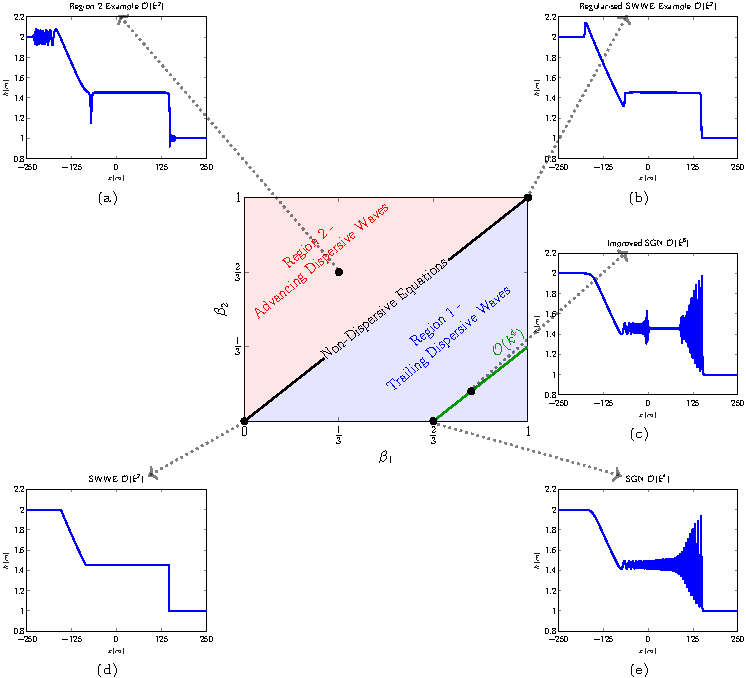
\includegraphics[width=\textwidth]{./Figures/Simulations/Comparison/3x3Grid.pdf}
	\caption{Phase speed regions of gSGNE in terms of $\left(\beta_1,\beta_2\right)$ showing important equations, their associated dispersion relationship accuracy \eqref{eq:DispWaterPower} and an example numerical solution for the dam-break problem \eqref{eqn:DB_Init} solved using $\left(1/3,2/3\right)$ in (a), $\left(1,1\right)$ in (b), $\left(2/3 + 2/15,2/15\right)$ in (c), $\left(0,0\right)$ in (d) and $\left(2/3 ,0\right)$ in (e).  }
	\label{Fig:WaveSpeedRegGrid}
\end{figure}


%-------------------------------------------------
\subsection{Alternative Conservative Form of the gSGNE}
%-------------------------------------------------
\citet{Clamond-Dutykh-2018-237} provided a reformulation of \eqref{eq:gSGNEuh} for the gSGNE, in an analogous to the way the SGNE \cite{Zoppou-etal-2017,Hank-etal-2010-2034,Li-2014-169} were reformulated. The purpose of this reformulation is to remove the mixed spatial-temporal derivative in the flux term of the momentum equation \eqref{eq:gSGNEuh}, which is difficult to treat numerically. This reformulation is obtained by introducing a new conserved quantity
\begin{gather*}
G = hu - \frac{\beta_1}{2} \dfrac{\partial }{\partial x} \left ( h^3 \dfrac{\partial u}{\partial x} \right )
\end{gather*}
and thus \eqref{eq:gSGNEuh} can be written in conservation law form for $G$ as
\begin{gather*}\label{eq:G_momentum}
\dfrac{\partial G }{\partial t}  + \dfrac{\partial}{\partial x} \left ( uG + \dfrac{gh^2}{2} - \beta_1 h^3\dfrac{\partial u}{\partial x}\dfrac{\partial u}{\partial x}  - \frac{1}{2} \beta_2 g h^2  \left[h\frac{\partial^2 h}{\partial x^2} + \frac{1}{2}\frac{\partial h}{\partial x}\frac{\partial h}{\partial x}\right]\right ) = 0
\end{gather*}
When $\beta_1 = 2/3$ then $G$ is the same conserved quantity introduced for the SGNE \cite{Zoppou-etal-2017,Hank-etal-2010-2034,Li-2014-169}.

This reformulation, provides the gSGNE in conservation law form for both $h$ and the new conserved quantity $G$. Thus the conservative gSGNE are
\begin{subequations}
\begin{align}
\dfrac{\partial h}{\partial t} &+ \dfrac{\partial (uh)}{\partial x} = 0  \label{eq:gSGNE_Gh} \\
\dfrac{\partial G }{\partial t} & + \dfrac{\partial}{\partial x} \left ( uG + \dfrac{gh^2}{2} - \beta_1 h^3\dfrac{\partial u}{\partial x}\dfrac{\partial u}{\partial x}  - \frac{1}{2} \beta_2 g h^2  \left[h\frac{\partial^2 h}{\partial x^2} + \frac{1}{2}\frac{\partial h}{\partial x}\frac{\partial h}{\partial x}\right]\right ) = 0.
\label{eq:gSGNE_GG}
\end{align}
with
\begin{gather}\label{eq:G_divergent}
G = uh - \frac{\beta_1}{2}\dfrac{\partial }{\partial x} \left ( h^3 \dfrac{\partial u}{\partial x} \right ).
\end{gather}
\label{eq:gSGNE_G}
\end{subequations}

Now that the gSGNE are written in conservation law form and have a bound on the phase speeds, they can be solved numerically using the hybrid finite volume technique described by \citet{Zoppou-etal-2017} for the SGNE.

\section{Numerical Scheme}
The proposed numerical scheme for the gSGNE extends those previously published for the SGNE \cite{Zoppou-etal-2017,Hank-etal-2010-2034} to allow any $\beta$ values and the associated additional terms. We begin the description of the numerical scheme by giving a brief outline of the finite volume method and the discretisation therein. We then provide an overview of the numerical technique and then describe the simplest second-order implementation of this scheme in detail. With previous studies \cite{Zoppou-etal-2017,Pitt-2019} showing the sufficiency and necessity of second-order methods for the SGNE. 

\subsection{Finite Volume Method and Discretisation}
The core of these hybrid finite volume methods for the gSGNE is the finite volume method used to solve the equations in conservation law form. The finite volume method solves equations of the form 
\begin{equation}
\label{eqn:Conservf}
\frac{\partial q}{\partial t} + \frac{\partial f(q)}{\partial x} = 0
\end{equation}
where $q$ is a generic conserved quantity. This is the form of the gSGNE after the reformulation \eqref{eq:gSGNE_G}. In the finite volume method \eqref{eqn:Conservf} is integrated over cells of fixed width $\Delta x$ in space and over time steps of fixed length $\Delta t$.  The midpoint of the $j^{th}$ cell is given by $x_j = x_0 + j \Delta x$ while the cell edges of the $j^{th}$ cell are given by $x_{j-1/2} = x_0 + (j - \frac{1}{2}) \Delta x$ and $x_{j+1/2} = x_0 + (j + \frac{1}{2}) \Delta x$. Likewise the $n^{th}$ time step is given by $t^n = t^0 + n \Delta t$. 

Integrating \eqref{eqn:Conservf} over both space and time results in
\begin{equation}
\bar{q}^{n+1}_j = \bar{q}^{n}_j  +  \dfrac{\Delta t}{\Delta x}\left[F^n_{j+1/2} - F^n_{j-1/2}\right]
\label{eqn:ConsFVM}
\end{equation}
where 
\begin{equation*}
\bar{q}^n_j = \frac{1}{\Delta x} \int_{x_j - \Delta x / 2}^{x_j - \Delta x / 2} q(x,t^n) \; dx
\end{equation*}
is the average of $q$ over the $j^{th}$ cell at time $t^n$ and   
\begin{equation*}
F^n_{j\pm 1/2} =\frac{1}{\Delta t} \int_{t^n}^{t^{n+1}} f(q(x_{j\pm 1/2},t)) dt
\end{equation*}
is the average flux of $q$ across the cell edge from time $t^n$ to $t^{n+1}$. Therefore, if $F^n_{j\pm 1/2}$ can be approximated with the appropriate order of accuracy, then we have an explicit method for updating the cell average of the conserved quantities through time for equations in conservation law form \eqref{eqn:Conservf}. In this paper we only consider approximations to $F^n_{j\pm 1/2}$ which are first-order accurate in time. 


\subsection{Overview}
\label{subsec:Overview}
We will now describe the numerical scheme, which uses the above finite volume formulation to solve \eqref{eq:gSGNE_Gh} and \eqref{eq:gSGNE_GG}. When describing this broad overview it is also useful to consider collections of the point-wise values $q$ or cell averaged values $\bar{q}$ described above over the whole domain at a particular time. Thus for $q$, we define $\vecn{q}^n$ to be the vector of $q^n_j$ values and $\bar{\vecn{q}}^n$ to be the vector of $\bar{q}^n_j$ values for all cells in the domain at time $t^n$. 

The numerical scheme for the gSGNE based on the finite volume method \eqref{eqn:ConsFVM} then proceeds as follows. Begin at the $n^{th}$ time step where the vectors of cell averages of the conserved quantities $\bar{\vecn{h}}^n$ and $\bar{\vecn{G}}^n$ are either known or provided as initial conditions. 
\begin{enumerate}
	\item Solve \eqref{eq:G_divergent} using $\bar{\vecn{h}}^n$ and $\bar{\vecn{G}}^n$ to obtain an approximation to $\bar{{\vecn{u}}}^n$, which can be expressed as
	\[\mathcal{A}\left(\bar{\vecn{h}}^n,\bar{\vecn{G}}^n\right) \boldsymbol{\rightarrow} \bar{{\vecn{u}}}^n.\]
	\item Solve \eqref{eq:gSGNE_Gh} and \eqref{eq:gSGNE_GG}, using the finite volume method \eqref{eqn:ConsFVM} with an approximate Riemann solver such as the one described by \citet{Kurganov-etal-2001-707}, to obtain $\bar{h}^{n+1}_j$ and $\bar{G}^{n+1}_j$ at the next time step, like so
	\[\mathcal{F}\left(\bar{\vecn{h}}^n,\bar{\vecn{G}}^n,\bar{{\vecn{u}}}^n\right) \boldsymbol{\rightarrow}\bar{\vecn{h}}^{n+1 },\bar{\vecn{G}}^{n+1}.\]
	\item Since $\mathcal{F}$ is only first-order accurate in time, Steps 1 and 2 are repeated and combined using a convex combination to obtain a Strong Stability Preserving (SSP) Runge Kutta time stepping method \cite{Gottlieb-etal-2003-89} to approximate $\bar{\vecn{h}}^{n+1 }$ and $\bar{\vecn{G}}^{n+1}$ with the correct accuracy in time. 
\end{enumerate}

This numerical scheme produces the numerical methods of \citet{Hank-etal-2010-2034}, \citet{Zoppou-etal-2017} and \citet{Pitt-2019} when $\beta_1 = 2/3$ and $\beta_2 = 0$. Additionally, when $\beta_1 = \beta_2 = 0$ the gSGNE reduces to the SWWE, and this numerical scheme reduces to a traditional finite volume method \cite{Roberts-2003-129}.  

\subsection{Example Implementation}
To demonstrate the utility of this numerical scheme we present a simple second-order implementation, and then validate it in the following section. The description of this numerical method will be broken up into the steps described in Section \ref{subsec:Overview} for simplicity and also to highlight the interchangeability of the different parts of the scheme.

\subsubsection{Step 1 - Solution of the Elliptic Equation}
To solve \eqref{eq:G_divergent} given $\bar{\vecn{h}}^n$ and $\bar{\vecn{G}}^n$ to obtain $\bar{\vecn{u}}^n$ we use the observation that the cell average and the cell nodal value are equal up to second-order accuracy, so that $\bar{\vecn{q}}^n = {\vecn{q}}^n + \mathcal{O}\left(\Delta x^2\right)$ for all the quantities of interest. Assuming that $u$ is sufficiently smooth, then a second-order central finite difference approximation can be used to accurately solve \eqref{eq:G_divergent}. 

The second-order central finite difference approximation to \eqref{eq:G_divergent} can be written as
\begin{equation}
{\vecn{u}}^n = \vecn{A}^{-1} {\vecn{G}}^n
\label{eq:FDGeqn}
\end{equation}
where $\vecn{A}$ is a tri-diagonal matrix with the sub-diagonal, diagonal and super-diagonal given by
\begin{subequations}
\begin{align}
A_{j,j-1} &=  -\frac{\beta_1}{2}  \left[  \dfrac{\left(h_j^n\right)^3}{\Delta x^2} -  \dfrac{3\left(h_j^n\right)^2}{2\Delta x} \dfrac{h_{j+1}^n - h_{j-1}^n}{2\Delta x}\right] \\
A_{j,j} &= h^n_j + \beta_1\dfrac{\left(h_j^n\right)^3}{\Delta x^2} \\
A_{j,j+1} &=  -\frac{\beta_1}{2}  \left[  \dfrac{\left(h_j^n\right)^3}{\Delta x^2} +  \dfrac{3\left(h_j^n\right)^2}{2\Delta x} \dfrac{h_{j+1}^n - h_{j-1}^n}{2\Delta x}\right]
\end{align}
\label{eq:Adiags}
\end{subequations}
respectively. 

The finite difference approximation \eqref{eq:FDGeqn} can be solved with any matrix solver, for this method we use the explicit Thomas Algorithm \cite{Conte-DeBoor-1980}. This is an efficient method provided $\vecn{A}$ is non-singular which is the case as long as $h_{j}^n > 0$, which is true for all the problems of interest in this paper. 

Thus as desired we have 
\begin{equation}
\mathcal{A}\left(\bar{\vecn{h}}^n,\bar{\vecn{G}}^n\right) = \vecn{A}^{-1} {\vecn{G}}^n = \vecn{u}^n \boldsymbol{\rightarrow} \bar{{\vecn{u}}}^n. 
\label{eq:A_secondord}
\end{equation}


\subsubsection{Step 2 -  Finite Volume Method  - Reconstruction}
The finite volume method of \citet{Kurganov-etal-2001-707} relies on approximations of all the terms in the spatial derivative of the flux at the cell edges $x_{j\pm1/2}$. Thus the following quantities require second-order approximations at the cell edges: $u$, $h$, $G$, $\partial u / \partial x$, $\partial h / \partial x$, $\partial^2 h / \partial x^2$. In this paper we are interested in validating the numerical method by reproducing solutions to smooth analytic and forced solutions for all members of the gSGNE. We are also interested in validating the numerical method for the discontinuous dam-break solution for only the SWWE where $\beta_1 = \beta_2 = 0$ and thus only $h$, $u$ and $G = uh$ need to be approximated. For this reason our gSGNE solver uses approximations to  $u$, $h$, $G$ that allow for discontinuities and thus use limiting. Whereas the approximations to the derivatives $\partial u / \partial x$, $\partial h / \partial x$, $\partial^2 h / \partial x^2$ will assume that these quantities are smooth and thus do not require limiting. 

Figure \ref{Fig:WaveSpeedRegGrid} demonstrates the adequacy of this reconstruction approach even in situations where the derivatives are present in the equations but are not smooth. A main reason for this is that the elliptic equation \eqref{eq:G_divergent} helps control the smoothness of $u$. However, this does not explain why we get reasonable results when assuming the derivatives of $h$ are smooth when they are not smooth in the initial conditions. For the validations performed in this paper, the assumption on the smoothness of the derivatives $\partial u / \partial x$, $\partial h / \partial x$, $\partial^2 h / \partial x^2$ is adequate.


The reconstructions for $u$, $h$ and $G$ can be summarised for a general quantity $q$ like so
\begin{align}
q^+_{j-1/2} = \bar{q}_j - \frac{\Delta x}{2} s_j & & \text{and} & &
q^-_{j+1/2} = \bar{q}_j + \frac{\Delta x}{2} s_j
\end{align}
where
\begin{equation}
s_j = \text{minmod}\left(\theta \dfrac{\bar{q}_j - \bar{q}_{j-1}}{\Delta x},  \dfrac{\bar{q}_{j+1} - \bar{q}_{j-1}}{2\Delta x},\theta \dfrac{\bar{q}_{j+1} - \bar{q}_{j}}{\Delta x}\right).
\end{equation}
The minmod function is defined as follows
\begin{equation}
\text{minmod}\left(a,b,c\right) = \left\lbrace \begin{array}{l c l}
\min{\left(a,b,c\right)} & \text{when} & a<0, b<0, c<0 \\
\max{\left(a,b,c\right)} & \text{when} & a>0, b>0, c>0 \\
0 & & \text{otherwise}
\end{array} \right. . 
\end{equation}
This gives a reconstruction at each cell edge, so cell $j$ gives rise to $q^+_{j-1/2}$ and $q^-_{j+1/2} $ while cell $j+1$ gives rise to $q^+_{j+1/2}$ and $q^-_{j+3/2}$, all of which are required in the flux approximation.

For $\partial u / \partial x$, $\partial h / \partial x$ and $\partial^2 h / \partial x^2$ we assume that the quantities are smooth, and so using the appropriate order finite difference approximation at the cell edges is sufficient. We demonstrate these approximations for $x_{j+1/2}$ and a generic quantity $q$

\begin{align*}
\left[\dfrac{\partial q}{\partial x} \right]_{j+1/2} &= \dfrac{q_{j+1} - q_j}{\Delta x}, \\
\left[\dfrac{\partial^2 q}{\partial x^2} \right]_{j+1/2} &=  \dfrac{q_{j+2} - q_{j+1} - q_j + q_{j-1}}{2 \Delta x^2} .
\end{align*}


\subsubsection{Step 2 -  Finite Volume Method - Flux Approximation}
To solve \eqref{eq:gSGNE_Gh} and \eqref{eq:gSGNE_GG} which are both in conservation law form \eqref{eqn:Conservf} we use \eqref{eqn:ConsFVM}. Since we begin with $\bar{\vecn{h}}^n$ and $\bar{\vecn{G}}^n$, we only require an approximation to $F^n_{j\pm1/2}$ to obtain $\bar{\vecn{h}}^{n+1}$ and $\bar{\vecn{G}}^{n+1}$.

In this numerical scheme the approximate Riemann solver described by \citet{Kurganov-etal-2001-707} is used to calculate $F^n_{j\pm1/2}$. The major advantage of this scheme is that it only requires bounds on the phase speeds. Only the calculation of the flux term $F^n_{j+1/2}$ is demonstrated as the process to calculate the flux term $F^n_{j-1/2}$ is identical but with different cells. For $q$ the flux is approximated by
\begin{equation}\label{eqn:HLL_flux}
F^n_{j+\frac{1}{2}} = \dfrac{a^+_{j+\frac{1}{2}} f\left(q^-_{j+\frac{1}{2}}\right) - a^-_{j+\frac{1}{2}} f\left(q^+_{j+\frac{1}{2}}\right)}{a^+_{j+\frac{1}{2}} - a^-_{j+\frac{1}{2}}}  + \dfrac{a^+_{j+\frac{1}{2}} \, a^-_{j+\frac{1}{2}}}{a^+_{j+\frac{1}{2}} - a^-_{j+\frac{1}{2}}} \left [ q^+_{j+\frac{1}{2}} - q^-_{j+\frac{1}{2}} \right ]
\end{equation}

where $a^+_{j+\frac{1}{2}}$ and $a^-_{j+\frac{1}{2}}$ are given by the phase speed bounds and all quantities on the right hand side are computed at time $t^n$. Applying the phase speed bounds \eqref{eq:wavespeedbound1} and \eqref{eq:wavespeedbound2} we obtain
\begin{align}
a^-_{j+\frac{1}{2}} &= \min\left\lbrace 0\;,\;  u^-_{j + 1/2} - \max{\left(1 , \sqrt{\frac{\beta_2}{\beta_1}}\right)} \sqrt{g h^-_{j + 1/2}}  \;,\;u^+_{j + 1/2} -\max{\left(1 , \sqrt{\frac{\beta_2}{\beta_1}}\right)} \sqrt{g h^+_{j + 1/2}} \right\rbrace  ,\\
a^+_{j+\frac{1}{2}} &= \max\left\lbrace 0 \;,\;  u^-_{j + 1/2} + \max{\left(1 , \sqrt{\frac{\beta_2}{\beta_1}}\right)}\sqrt{g h^-_{j + 1/2}}  \;,\;u^+_{j + 1/2} + \max{\left(1 , \sqrt{\frac{\beta_2}{\beta_1}}\right)}\sqrt{g h^+_{j + 1/2}} \right\rbrace
\label{eqn:WaveSpeedBoundsFluxApprox}
\end{align}
where the $\max{\left(1 , \sqrt{{\beta_2}/{\beta_1}}\right)}$ accounts for the different phase speed bounds  \eqref{eq:wavespeedbound1} and \eqref{eq:wavespeedbound2}, which depend on the choice of $\beta$ values. 

The flux functions $f(q^-_{j+\frac{1}{2}})$ and $f(q^+_{j+\frac{1}{2}})$ are evaluated using the reconstructed values of the $j^{th}$ and $(j+1)^{th}$ cell respectively. From the continuity equation \eqref{eq:gSGNE_Gh} we have
\begin{align*}
f\left(h^\pm_{j+\frac{1}{2}}\right) &= u^\pm_{j + 1/2}  h^\pm_{j + 1/2}.
\end{align*}

For the evolution of $G$ equation \eqref{eq:gSGNE_GG} we have 
\begin{multline}
f\left(G^\pm_{j+\frac{1}{2}}\right) =  u^\pm_{j + 1/2} G^\pm_{j + 1/2}  + \frac{g}{2}\left(h^\pm_{j + 1/2} \right)^2 - \beta_1\left(h^\pm_{j + 1/2}\right)^3 \left(\left[\frac{\partial {u}}{\partial x} \right]_{j + 1/2} \right)^2 \\ - \frac{1}{2} \beta_2 g \left(h^\pm_{j + 1/2}\right)^2  \left[h^\pm_{j + 1/2}\left[\dfrac{\partial^2 h}{\partial x^2} \right]_{j+1/2} + \frac{1}{2}\left(\left[\dfrac{\partial h}{\partial x} \right]_{j+1/2}\right)^2\right]
\end{multline}
where the derivatives are assumed to be smooth across the cell edge, and thus do not require different superscripts.

Since the reconstructions were given above for all these quantities, we can approximate $F^n_{j\pm1/2}$ using \eqref{eqn:HLL_flux} and thus employ \eqref{eqn:ConsFVM} to obtain $\bar{\vecn{h}}^{n+1}$ and $\bar{\vecn{G}}^{n+1}$ resulting in
\begin{equation}
\mathcal{F}\left(\bar{\vecn{h}}^n,\bar{\vecn{G}}^n,\bar{{\vecn{u}}}^n\right) =   \bar{q}^{n}_j  +  \dfrac{\Delta t}{\Delta x}\left[F^n_{j+1/2} - F^n_{j-1/2}\right] \boldsymbol{\rightarrow} \bar{\vecn{h}}^{n+1 },\bar{\vecn{G}}^{n+1}
\label{eq:F_secondord}
\end{equation}
as desired. 

\subsubsection{Step 3 - Runge-Kutta Time Stepping}
Combining both Steps 1 and Steps 2, provides a spatially second-order scheme with first-order time stepping. To arrive at a fully second-order method, we repeat Steps 1 and Steps 2 according to the second-order SSP Runge Kutta method \cite{Gottlieb-etal-2003-89}. Doing this we obtain the following scheme making use of the above implementation of $\mathcal{A}$, \eqref{eq:A_secondord} and $\mathcal{F}$, \eqref{eq:F_secondord}
\begin{align*}
\bar{\vecn{h}}^{(1)},\bar{\vecn{G}}^{(1)} &= \mathcal{F}\left(\bar{\vecn{h}}^n,\bar{\vecn{G}}^n,\mathcal{A}\left(\bar{\vecn{h}}^n,\bar{\vecn{G}}^n\right) \right) \\
\bar{\vecn{h}}^{(2)},\bar{\vecn{G}}^{(2)} &= \mathcal{F}\left(\bar{\vecn{h}}^{(1)},\bar{\vecn{G}}^{(1)},\mathcal{A}\left(\bar{\vecn{h}}^{(1)},\bar{\vecn{G}}^{(1)}\right) \right)\\
\bar{\vecn{h}}^{n+1},\bar{\vecn{G}}^{n+1} &= \frac{1}{2}\left(\bar{\vecn{h}}^n + \bar{\vecn{h}}^{(2)} \right) ,  \frac{1}{2}\left(\bar{\vecn{G}}^n + \bar{\vecn{G}}^{(2)} \right). 
\end{align*}
obtaining a stable fully second-order method for solving \eqref{eq:gSGNE_G}. 

\subsection{Boundary Conditions}
For the purposes of the validation below and for simplicity, we have applied Dirichlet boundary conditions using ghost cells over which the values of $h$, $G$ and $u$ are known. Thus in addition to the $m$ cells inside the boundary we have an additional $l$ cells either side of it so that we have the left ghost cells $-l$, $-l + 1$, $\dots$, $-1$ and the right ghost cells $m$, $m+1$, $\dots$, $m + l -1$. Since the numerical method has a maximum stencil that extends $2$ cells beyond the target cell, then $l$ must be greater than $1$. 

This boundary condition is applied to Step 1 by extending the matrix equation \eqref{eq:FDGeqn} to vectors containing the ghost cells $\vecn{\hat{u}}^n$ and $\vecn{\hat{G}}^n$ like so
\begin{align*}
\vecn{\hat{u}}^n &= \left[u^n_{-l} \; \dots \; u^n_{-1} \; u^n_{0}\; \dots \; u^n_{m-1}\; u^n_{m} \; \dots \; u^n_{m + l -1}   \right]^T \\
\vecn{\hat{G}}^n &= \left[G^n_{-l} \; \dots \; G^n_{-1} \; G^n_{0}\; \dots \; G^n_{m-1}\; G^n_{m} \; \dots \; G^n_{m + l -1}   \right]^T.
\end{align*}

Likewise the associated extended matrix $\vecn{\hat{A}}$ in \eqref{eq:FDGeqn} is the same as $\vecn{A}$ when $0 \le j \le m -1$  \eqref{eq:Adiags} with the additional associated ghost cell values given by
\begin{equation*}
\hat{A}_{j,j-1} =  0  \quad \quad
\hat{A}_{j,j} = 1 \quad \quad
\hat{A}_{j,j+1} = 0
\end{equation*}
when $j < 0$ or $j > m -1$. 

For Step 2 there is no need to reconstruct the quantities inside the ghost cells because $h$, $G$ and $u$ are given. 


\subsection{Courant-Frederichs-Lewy Condition}
To ensure the stability of the finite volume method \eqref{eqn:ConsFVM} the Courant-Friedrichs-Lewy (CFL) condition \cite{Courant-etal-1967-215} is used. The CFL condition is necessary for stability and ensures that time steps are small enough so that information is only transferred between neighbouring cells. For the gSGNE the CFL condition is 
\begin{equation}
\Delta t \le \frac{Cr }{\max_{j} \left\lbrace a^\pm_{j+1/2} \right\rbrace} \Delta x
\label{eqn:CFLcond}
\end{equation}
where $a^\pm_{j+1/2} $ are the phase speed bounds used in the flux approximation \eqref{eqn:WaveSpeedBoundsFluxApprox} and $0\le Cr \le 1$ is the Courant number. 

\section{Validation}
The numerical method described above is validated using analytic solutions for particular $\beta$ values that correspond to the SGNE and the SWWE as well as a forced solution. Together these tests demonstrate the ability of the method to reproduce analytic solutions to important members of the gSGNE family, as well as assessing the accuracy of the numerical method's approximation of all terms in the gSGNE.

\subsection{Convergence and Conservation Measures}
To validate the numerical solutions we make use of measures of convergence and conservation. The measure of convergence will be the relative deviation of the numerical solution from the equivalent analytic or forced solution using the $L_2$ norm. While the conservation properties of the numerical method will be measured by numerically approximating the energy in the initial conditions and the numerical solution and comparing them using a measure called $C_1$.

For a quantity $q$ with a vector of its analytic or forced solution at the cell midpoints $\vecn{q}$ and the numerical solution at the cell midpoints $\vecn{q}^*$, the discrete non-dimensional $L_2$ norm is
\begin{equation}
\label{eqn:Conv_Error}
L_2\left(\vecn{q},\vecn{q}^*\right) = \left( \dfrac{\displaystyle\sum_{j}^{}  \left(q_j - q^*_j\right)^2}{\displaystyle\sum_{j}^{}  q_j^2 } \right)^{\dfrac{1}{2}}
\end{equation}
where the time-step superscripts were suppressed for simplicity.

For a quantity $q$ with a vector of its values at the $n^{th}$ time step $\vecn{q}^n$, the total amount of the quantity is approximated by $C(\vecn{q}^n)$. The method for this is the same as the method described by \citet{Zoppou-etal-2017}, which has a higher order of accuracy than the numerical method used to solve the gSGNE. Using the numerical approximation to the total amounts, the conservation error is obtained using
\begin{equation}
\label{eqn:Cons_Error}
C_1\left(\vecn{q}^0,\vecn{q}^n\right) = \left \lbrace \begin{array}{l c r}
\dfrac{\left | C(\vecn{q}^0) - C(\vecn{q}^n) \right |}{\left| C(\vecn{q}^0) \right|} &,& \left| C(\vecn{q}^0) \right| > 0 \\ \\
\left | C(\vecn{q}^0) - C(\vecn{q}^n) \right |&,& \left| C(\vecn{q}^0) \right| = 0 
\end{array} \right. .
\end{equation}

%\begin{itemize}
%	\item Analytic solutions - we recover them (conservation and norm)
%	\item Forced solutions - our numerical method can handle any combination of beta values, all terms are approximated with correct order of accuracy. Limiters on gradients off. 
%\end{itemize}

\subsection{Analytic Solutions}
\label{sec:AnaSol}
The analytic solutions used to validate the numerical method, are the solitary travelling wave solution of the SGNE and the dam-break solution of the SWWE. The solitary travelling wave solution is a smooth travelling wave solution, where the non-linear and dispersive terms are in balance in the gSGNE. Whereas the dam-break solution of the SWWE demonstrates the robustness of the method in the presence of steep gradients. 

\subsubsection{SGNE - Solitary Travelling Wave Solution}
When $\beta_1 = 2/3$ and $\beta_2 = 0$ the gSGNE are equivalent to the SGNE which admit the following travelling wave solution \cite{El-etal-2006}
\begin{subequations}
	\begin{equation}
	h(x,t) = a_0 + a_1 \text{sech}^2\left( \kappa (x - ct) \right),
	\end{equation}
	\begin{equation}
	u(x,t) = c \left( 1- \dfrac{a_0}{h(x,t)} \right),
	\end{equation}
	where
	\begin{equation}
	\kappa = \dfrac{\sqrt{3a_1}}{2a_0 \sqrt{a_0 + a_1}}
	\end{equation}
	and
	\begin{equation}
	c = \sqrt{g\left(a_0 + a_1\right)}
	\label{eq:Sol_speed}
	\end{equation}
\end{subequations}
is the speed of the wave.

This travelling wave solution is maintained due to a balance between the dispersive terms and the non-linear terms in the momentum equation \eqref{eq:gSGNEuh}. This balance results in a solitary wave that is advected with a constant speed without a change in shape. Validating the numerical solutions for the gSGNE solver using this solution tests the balance between these terms in \eqref{eq:gSGNEuh}, and allows us to verify the method's conservation of energy as the solution is smooth. To enable a comparison between the numerical method and the SGNE solver of \citet{Zoppou-etal-2017} and \citet{Pitt-2019}, the chosen solitary travelling wave parameters were $a_0 = 1m$ and $a_1 = 0.7m$ and the acceleration due to gravity at the Earth's surface, $g = 9.81 m^2/s$ was used.

The numerical solution was solved over the domain $\left[-200m,200m\right]$ from $t=0s$ until $t=30s$. The spatial resolution was varied like so $\Delta x = 400 / (100 \times 2^{l})$, where $l$ was increased from $0$ to $12$. To satisfy the CFL condition \eqref{eqn:CFLcond} the time step $\Delta t = \Delta x  / ( 2 \sqrt{g(a_0 + a_1)})$ was chosen. The limiting parameter $\theta = 1.2$, was chosen to match previous numerical experiments \cite{Zoppou-etal-2017,Pitt-2019}.

Example numerical solutions for $h$, $u$ and $G$ with $\Delta x = 400 / (100 \times 2^{6}) \approx 0.06m$ are plotted in Figure \ref{Fig:Sol_Ex}. These examples demonstrate that the numerical solutions can reproduce the analytic solutions well.
%
\begin{figure}
	\centering
	\begin{subfigure}{0.32\textwidth}
		\centering
		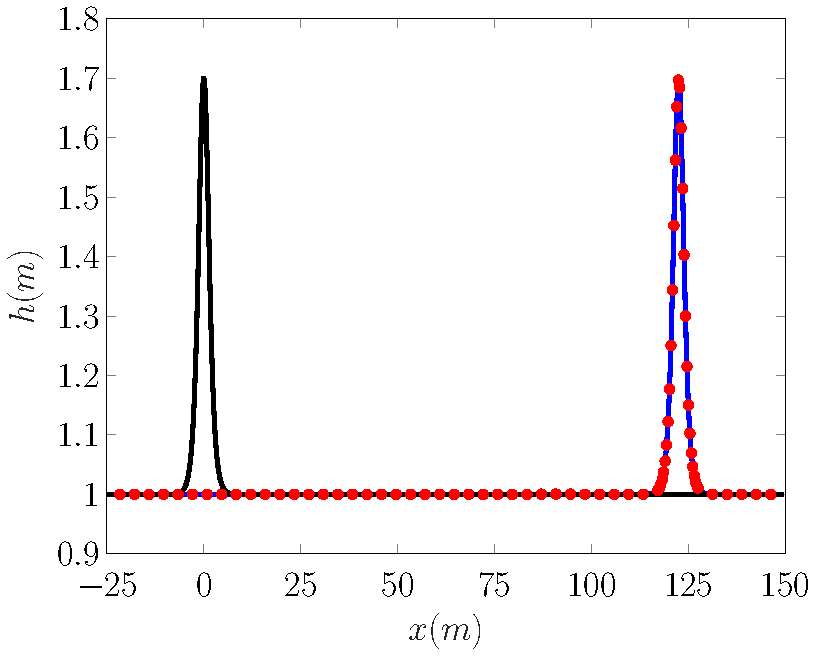
\includegraphics[width=\textwidth]{./Figures/Simulations/Validation/Serre/hEx.pdf}
		\caption{$h$}
	\end{subfigure}
	\begin{subfigure}{0.32\textwidth}
		\centering
		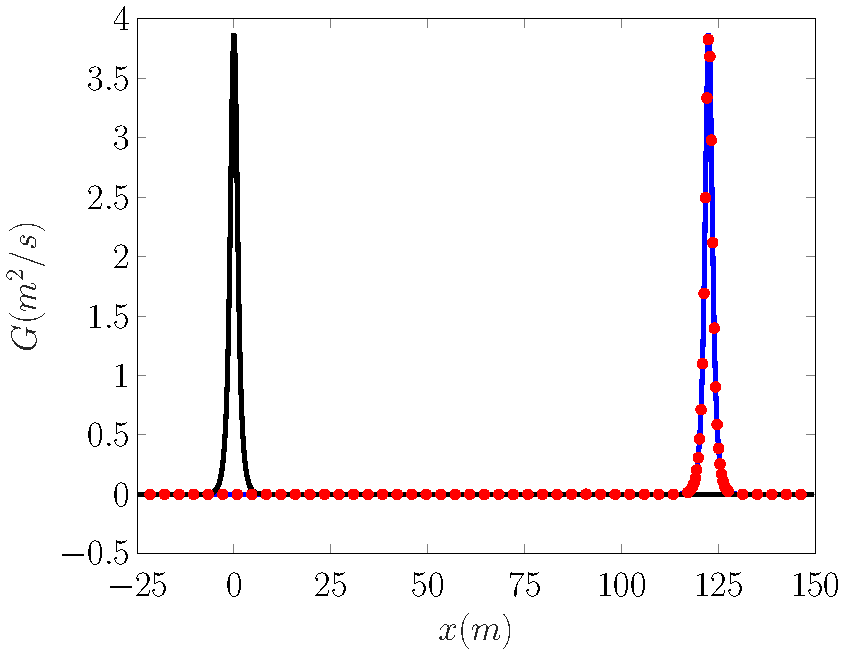
\includegraphics[width=\textwidth]{./Figures/Simulations/Validation/Serre/GEx.pdf}
		\caption{$G$}
	\end{subfigure}
	\begin{subfigure}{0.32\textwidth}
		\centering
		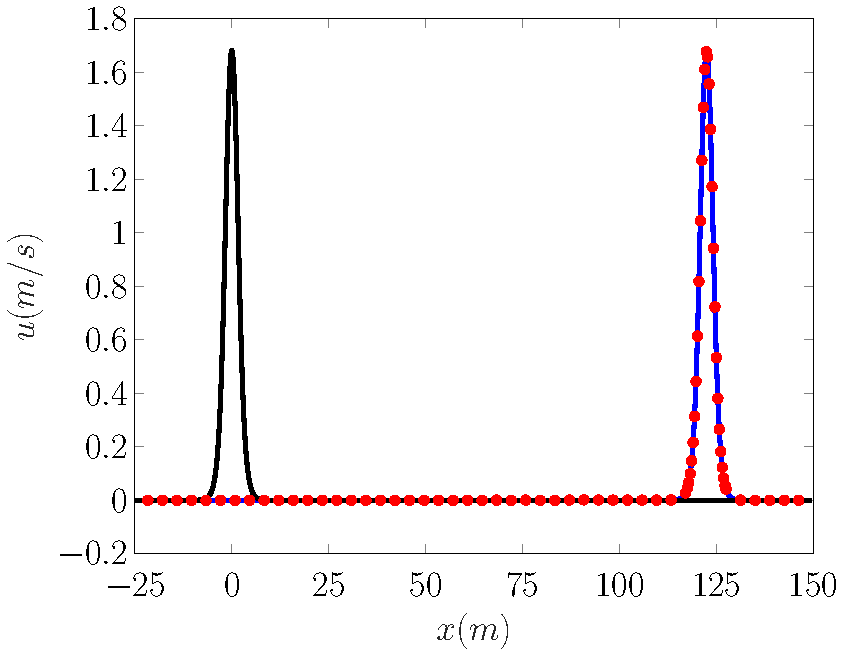
\includegraphics[width=\textwidth]{./Figures/Simulations/Validation/Serre/uEx.pdf}
		\caption{$u$}
	\end{subfigure}
	\caption{Plot of comparing initial (\solidrule), analytic solution ({\color{blue}\solidrule}), and numerical solution with $\Delta x \approx 0.06m$ (\tikzcircle{red}) at $t = 30s$.}
	\label{Fig:Sol_Ex}
\end{figure}

The convergence properties of the method as $\Delta x$ varies are given in Figure \ref{Fig:Sol_Comp}
where Figure \ref{Fig:Sol_Comp_Conv} shows the $L_2$ norm calculated over the whole domain and Figure \ref{Fig:Sol_Comp_Peak} shows the $L_2$ norm at the peak only. The $L_2$ norm over the whole domain demonstrates that all quantities are approximated with second-order accuracy, and thus the method is second-order accurate. The $L_2$ norm at the peak was measured by taking the relative difference between the numerical solutions value at the peak of the wave which are given by $\max\left({\vecn{h}^n}\right)$, $\max\left({\vecn{u}^n}\right)$ to the analytic values which are $a_0 + a_1$ and $c a_0 / \left(a_0 + a_1\right)$ respectively. The $L_2$ norm at the peak demonstrates that even with the slope limiting and the diffusion introduced by the flux approximation \cite{Pitt-2018-61}, the numerical method introduces little diffusion and is second-order accurate. 
%
\begin{figure}
	\centering
	\begin{subfigure}{0.49\textwidth}
		\centering
		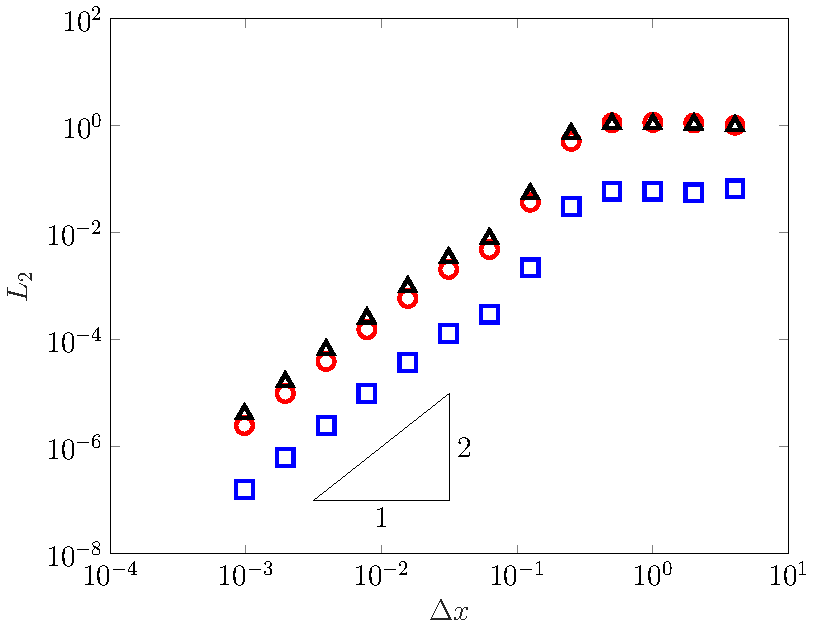
\includegraphics[width=\textwidth]{./Figures/Simulations/Validation/Serre/NormResults.pdf}
		\caption{Whole Domain}
		\label{Fig:Sol_Comp_Conv}
	\end{subfigure}
	\begin{subfigure}{0.49\textwidth}
		\centering
		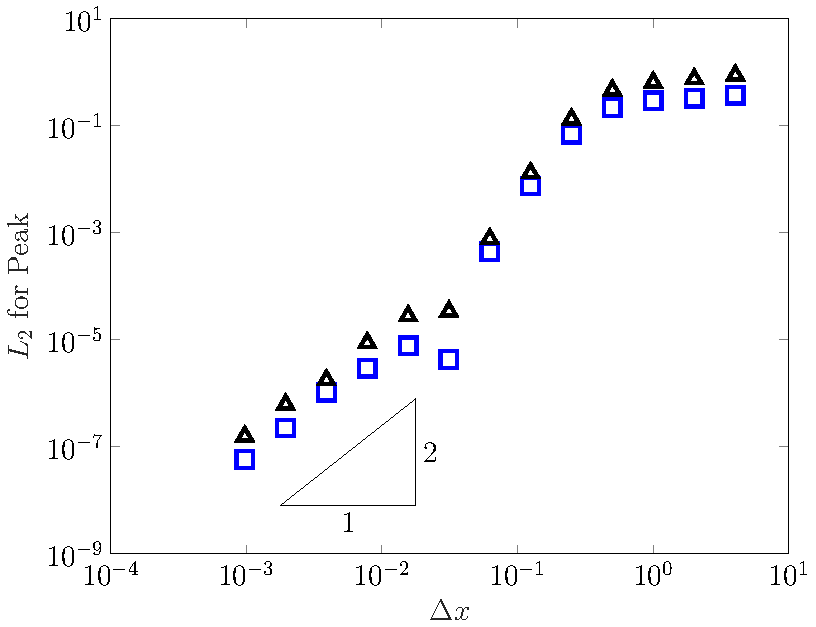
\includegraphics[width=\textwidth]{./Figures/Simulations/Validation/Serre/PeakError.pdf}
		\caption{Peak Only}
		\label{Fig:Sol_Comp_Peak}
	\end{subfigure}
	\caption{Convergence plots for $h$ (\squaret{blue}) , $G$ (\circlet{red}) and $u$ (\trianglet{black}) as $\Delta x$ varies.}
	\label{Fig:Sol_Comp}
\end{figure}

The conservation error $C_1$ \eqref{eqn:Cons_Error} of the numerical solutions as $\Delta x$ varies is given in Figure \ref{Fig:Sol_Comp_Cons}. This conservation measure demonstrates that the finite volume method conserves $h$ and $G$ up to round-off error, which accumulates as $\Delta x$ increases due to the additional number of calculations. Since $uh$ and $\mathcal{E}$ are not conserved quantities in our finite volume method which solves \eqref{eq:gSGNE_Gh} and \eqref{eq:gSGNE_GG}, they are not conserved up to round-off error. However, the conservation properties of $uh$ and $\mathcal{E}$ are good, with both exhibiting conservation errors that have better than second-order convergence in $\Delta x$. 
%
\begin{figure}
	\centering
	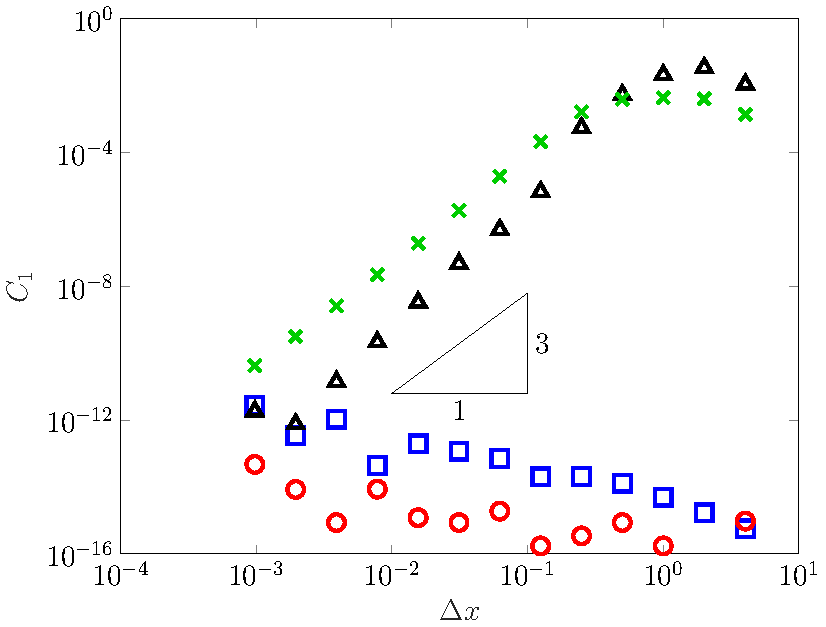
\includegraphics[width=0.49\textwidth]{./Figures/Simulations/Validation/Serre/EnergyResults.pdf}
	\caption{Conservation plot for $h$ (\squaret{blue}) , $G$ (\circlet{red}), $uh$ (\trianglet{black}) and $\mathcal{E}$ (\crosst{green!80!black}) as $\Delta x$ varies.}
	\label{Fig:Sol_Comp_Cons}
\end{figure}

By locating the cell on which $\vecn{h}^n$ achieves its maximum, we can provide an upper and lower bound for the speed of the numerical solution to the travelling wave problem where the lower bound is $c^*_{-}= (x_{\text{peak cell}} - 0.5 \Delta x) / t$ and the upper bound is $c^*_{+} = (x_{\text{peak cell}} + 0.5 \Delta x) / t$. These upper and lower bounds are compared to the analytic value $c$ given by \eqref{eq:Sol_speed} in Figure \ref{Fig:Sol_Comp_Speed}. This figure demonstrates the diffusion of the numerical scheme when $\Delta x$ is large because both the upper and lower bounds on the wave speed are below the analytic value. However, this diffusion becomes negligible when $\Delta x$ is small, and for the lowest $\Delta x$ value we observe that $ c^*_{-}< c  < c^*_{+}$, indicating that the peak is travelling at the correct speed up to cell width accuracy.
% 
\begin{figure}
	\centering
	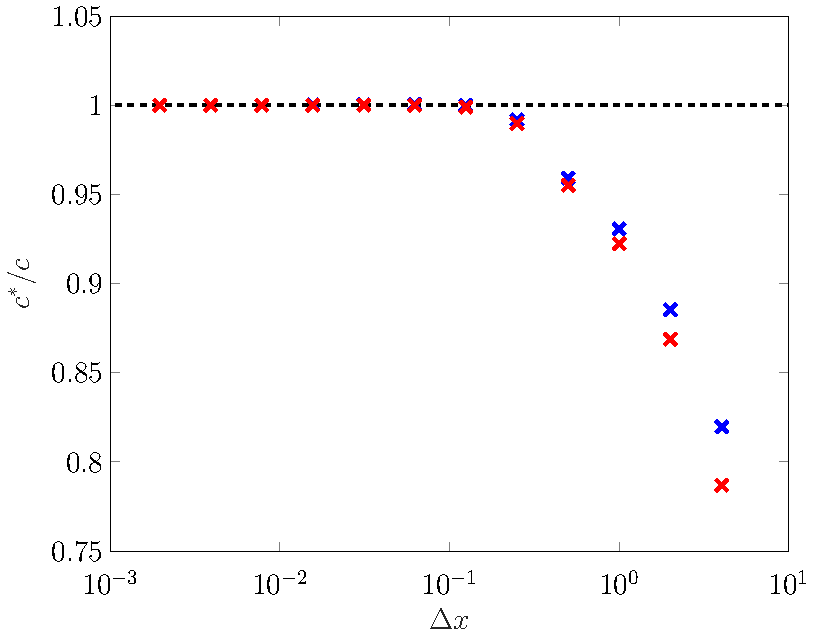
\includegraphics[width=0.49\textwidth]{./Figures/Simulations/Validation/Serre/PeakSpeedEstimates.pdf}
	\caption{Plot of $c^*_{+} / c $ (\crosst{blue}),  $c^*_{-} / c$ (\crosst{red}) and the analytic value (\dashedrule) as $\Delta x$ varies.}
	\label{Fig:Sol_Comp_Speed}
\end{figure}

These results agree well with the numerical solutions of \citet{Pitt-2019}, who compared various numerical methods for the SGNE. This demonstrates that the numerical method solving the gSGNE when $\beta_1 = 2/3$ and $\beta_2 = 0$ accurately reproduces the analytic solution of the SGNE.

\subsubsection{SWWE - Dam-break Solution }
When $\beta_1=\beta_2 =0$ the gSGNE equations reduce to the SWWE. Consequently, \eqref{eq:gSGNE_GG} and \eqref{eq:gSGNEuh} become identical with $G = uh$. The SWWE possess an analytic solution to the dam-break problem given by the initial conditions
\begin{subequations}
\begin{align}
h(x,0) & = \left\lbrace \begin{array}{c c}
h_0 & x < 0\\
h_1 & x \ge 0
\end{array} \right.  \\
u(x,0) &= 0 \\
G(x,0) &= 0.
\end{align}
\label{eqn:DB_Init}
\end{subequations}

The solution to the dam-break problem using the conservation of mass \eqref{eq:gSGNEh} and momentum \eqref{eq:gSGNEuh} equations is given by
\begin{subequations}
\begin{align}
h(x,t) &= \left \lbrace \begin{array}{l c r}
h_0 &,& x \le -t\sqrt{g h_0} \\
\frac{4}{9g} \left(\sqrt{gh_0} - \frac{x}{2t}\right)^2 &,&  -t\sqrt{g h_0} < x \le t \left(u_2 - \sqrt{g h_2}\right)  \\
h_2 &,&  t \left(u_2 - \sqrt{g h_2}\right) < x \le t S  \\
h_1 &,&   t S \le x \\
\end{array} \right.  \\
u(x,t) &= \left \lbrace \begin{array}{l c r}
0 &,& x \le -t\sqrt{g h_0} \\
\frac{2}{3} \left(\sqrt{gh_0} + \frac{x}{t}\right) &,&  -t\sqrt{g h_0} < x \le t \left(u_2 - \sqrt{g h_2}\right)  \\
u_2 &,&  t \left(u_2 - \sqrt{g h_2}\right) < x \le t S  \\
0 &,&   t S_2 \le x \\
\end{array} \right. .
\end{align}
\end{subequations}
%
The constant state values $h_2$ and $u_2$ and the shock speed $S$ can be calculated for any initial conditions by solving
\begin{subequations}
\begin{align}
\label{eq:SWWEMiddleState}
h_2 &= \dfrac{h_0}{2} \left(  \sqrt{1 + 8 \left( \dfrac{2 h_2}{h_2 - h_0} \left(\dfrac{\sqrt{gh_1} - \sqrt{gh_2}}{\sqrt{gh_0}}\right)\right)^2 } - 1 \right) \\
u_2 &= 2\left(\sqrt{gh_1} - \sqrt{gh_2} \right),\\
S &= \dfrac{2 h_2}{h_2 - h_1}\left(\sqrt{gh_0} - \sqrt{gh_2} \right). \label{eq:SWWEMiddleState_S2}
\end{align}
\end{subequations}

The initial conditions as well as the analytic solution are discontinuous. Due to the discontinuities the solutions to the initial conditions are not unique, as solving the momentum equation \eqref{eq:gSGNEuh} or the energy equation \eqref{eq:gSGNEE} results in solutions with similar structures but different shock speeds. The solution presented above is solution of the mass \eqref{eq:gSGNEh} and momentum \eqref{eq:gSGNEuh} equations, as these equations are the basis of the numerical method.

A number of numerical experiments were run for the dam-break problem with $h_0 = 2m$ and $h_1 = 1m$. The domain of the solution was $\left[-250m,250m\right]$ with a final time of $t=35s$.  The spatial resolution was varied like so $\Delta x = 500 / (100 \times 2^{l})$ where $l$ was increased from $0$ to $12$. To satisfy the CFL condition \eqref{eqn:CFLcond} the time step length $\Delta t = \Delta x  / \left( 2 \sqrt{g h_0}\right)$ was used. The limiting parameter $\theta = 1.0$ and the acceleration due to gravity $g = 9.81 m^2/s$ were used. 

Example numerical solutions with the spatial resolution $\Delta x = 500 / (100 \times 2^{5}) \approx  0.15m$ and the analytic solutions for $h$, $G$ and $u$ at the final time are plotted in Figure \ref{Fig:DB_Ex}. These figures demonstrate that the method is robust in the presence of steep gradients and accurately reproduces the analytic solution. 
%
\begin{figure}
	\centering
	\begin{subfigure}{0.32\textwidth}
		\centering
		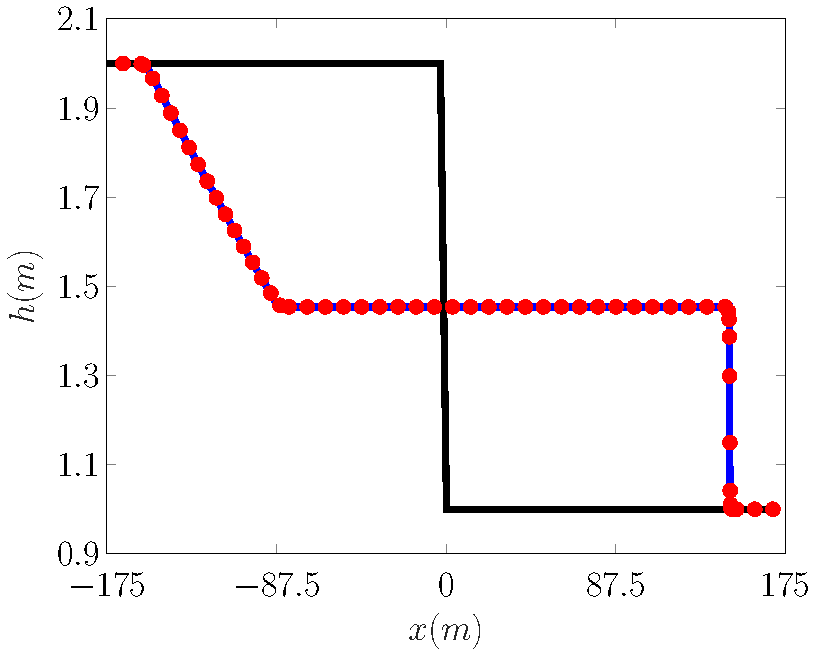
\includegraphics[width=\textwidth]{./Figures/Simulations/Validation/DBSWWE/hEx.pdf}
		\caption{$h$}
	\end{subfigure}
	\begin{subfigure}{0.32\textwidth}
		\centering
		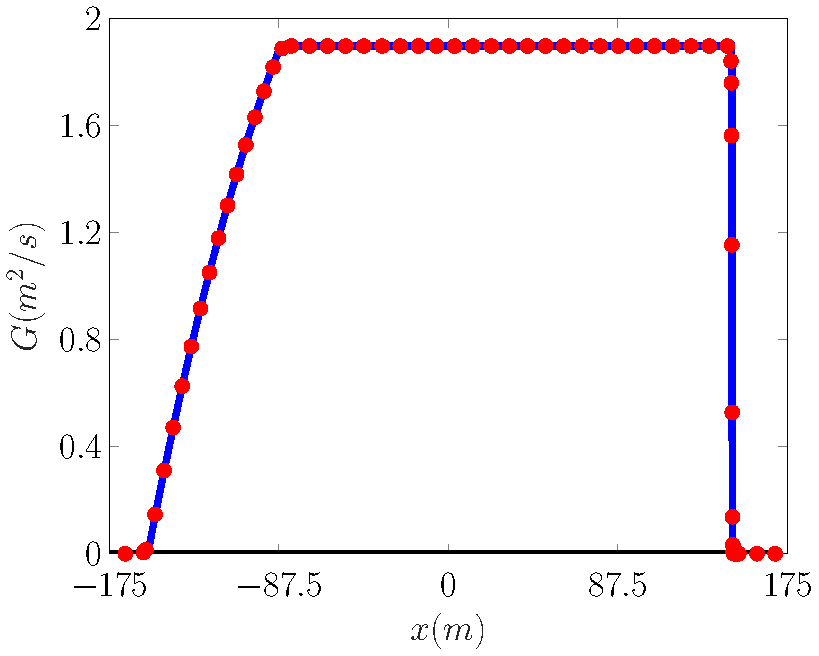
\includegraphics[width=\textwidth]{./Figures/Simulations/Validation/DBSWWE/GEx.pdf}
		\caption{$G = uh$}
	\end{subfigure}
	\begin{subfigure}{0.32\textwidth}
		\centering
		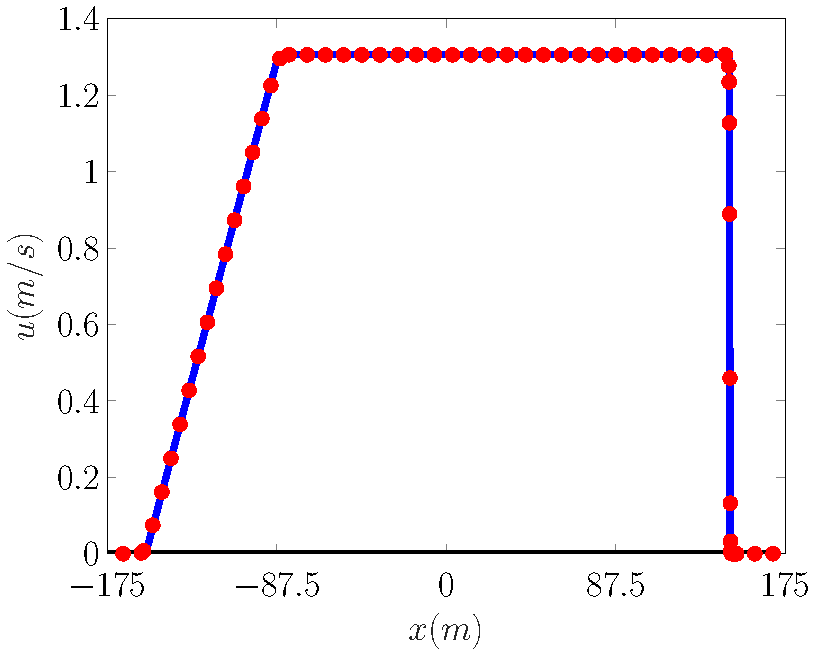
\includegraphics[width=\textwidth]{./Figures/Simulations/Validation/DBSWWE/uEx.pdf}
		\caption{$u$}
	\end{subfigure}
	\caption{Comparison of initial (\solidrule), analytic solution ({\color{blue}\solidrule}), and numerical solution with $\Delta x \approx 0.15m$ (\tikzcircle{red}) at  $t=35s$.}
	\label{Fig:DB_Ex}
\end{figure}

The presence of discontinuities in the analytic solution makes accurately assessing convergence of the numerical solutions difficult. To circumvent these issues, the convergence measure has been restricted to comparing the numerical and analytic solutions for the constant region between the rarefaction fan and the shock. This modified convergence measure as $\Delta x$ is varied is plotted in Figure \ref{Fig:DB_Comp_Conv}. This figure demonstrates that the scheme retains it's second-order accuracy away from discontinuities, as desired. 

Since the analytic solution contains discontinuities all three conservation laws for $h$, $G$ and $\mathcal{E}$ are not all satisfied simultaneously \cite{Pu-2018-1361}. Since we solved equations for $h$ and $G$, these quantities are conserved in the analytic solutions however, $\mathcal{E}$ is no longer conserved and energy is lost as the shock propagates. Therefore, we introduce a new measure $\mathcal{E}^*$ which measures the conservation error of the energy by comparing the total energy in the numerical solution with the total energy in the analytic solution at the final time. The conservation error for mass, momentum and energy as calculated normally and the new corrected energy are all compared in Figure \ref{Fig:DB_Comp_Cons}. This figure demonstrates that due to the use of the finite volume method even in the presence of discontinuities the conserved quantities $h$ and $G$ are conserved up to round-off error, leading to their conservation error increasing as $\Delta x$ decreases. Energy is not conserved by the analytic solution, and this can be seen as the conservation error of $\mathcal{E}$ does not improve as $\Delta x$ decreases. However, when accounting for the lack of energy conservation by using $\mathcal{E}^*$ we are able to recover first-order accuracy. Given that this solution contains a discontinuity these are good conservation results \cite{Shu-2012-59-5}. 
%
\begin{figure}
	\centering
	\begin{subfigure}{0.49\textwidth}
		\centering
		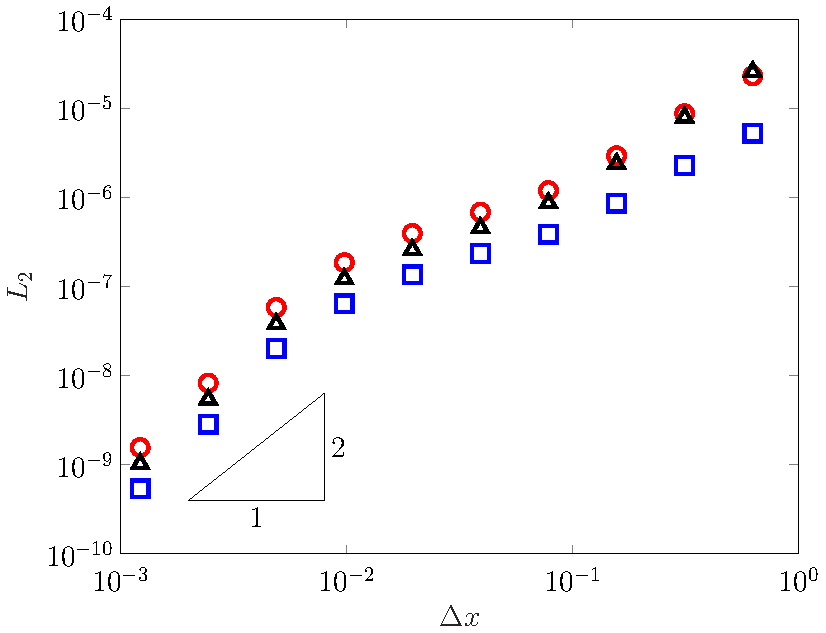
\includegraphics[width=\textwidth]{./Figures/Simulations/Validation/DBSWWE/ConvergenceInConstantState.pdf}
		\caption{$L_2$ for constant state for $h$ (\squaret{blue}) , $G$ (\circlet{red}) and $u$ (\trianglet{black})}
		\label{Fig:DB_Comp_Conv}
	\end{subfigure}
	\begin{subfigure}{0.49\textwidth}
		\centering
	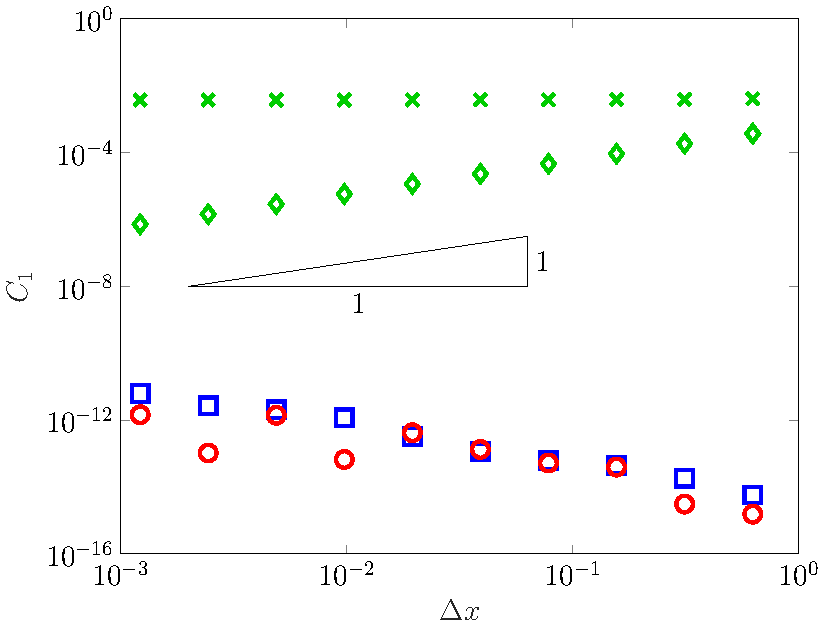
\includegraphics[width=\textwidth]{./Figures/Simulations/Validation/DBSWWE/EnergyResults.pdf}
\caption{$C_1$ for $h$ (\squaret{blue}), $G=uh$ (\circlet{red}), $\mathcal{E}$ (\crosst{green!80!black}) and $\mathcal{E}^*$ (\diamondt{green!80!black})}
		\label{Fig:DB_Comp_Cons}
	\end{subfigure}
	\caption{Convergence and conservation plots.}
	\label{Fig:DB_Comp}
\end{figure}

To further justify the ability of the method to resolve the discontinuous analytic solution, I have found lower $x_\text{lower}$ and upper $x_\text{upper}$ bounds for the location of the shock in the numerical solution and used this to bound the shock speed in the numerical solution. For $x_\text{lower}$ this was accomplished by finding the first cell with $\bar{h}_j \le h_1 + \frac{9}{10} \left(h_2 - h_1\right)$ and for $x_\text{upper}$ this was achieved by finding the first cell with $\bar{h}_j \le h_1 + \frac{1}{10} \left(h_2 - h_1\right)$. Consequently, the lower bound for the shock speed $S^*_{-} = x_\text{lower} / t$ and the upper bound for the shock speed $S^*_{+} = x_\text{upper} / t$ were calculated and compared to the analytic value $S$ given by \eqref{eq:SWWEMiddleState_S2} in Figure \ref{Fig:DB_ShockSpeed_Comp}. This figure demonstrates that as $\Delta x$ decreases the numerical solutions are better resolving the shock. Furthermore it demonstrates that $x_\text{lower}$ and $x_\text{upper}$ provide a bound for the true location of the shock. 
%
\begin{figure}
	\centering
	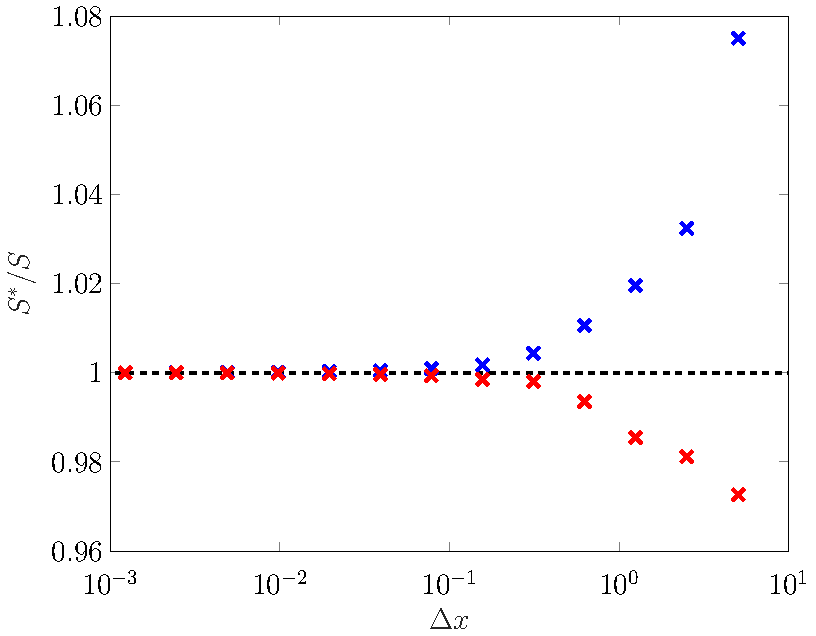
\includegraphics[width=0.5\textwidth]{./Figures/Simulations/Validation/DBSWWE/ShockSpeedEstimates.pdf}
	\caption{Plot of $S^*_{+} / S$ (\crosst{blue}),  $S^*_{-} / S$ (\crosst{red}) and analytic value (\dashedrule) as $\Delta x$ varies.}
	\label{Fig:DB_ShockSpeed_Comp}
\end{figure}

These results demonstrate that the analytic solution of the SWWE has been accurately reproduced by the numerical method which solves the gSGNE when $\beta_1 = \beta_2 = 0$. 

\subsection{Forced Solutions}
There are currently no known analytic solutions to the gSGNE for other $\beta$ values. Hence, to demonstrate the validity and versatility of the method to solve the gSGNE for other $\beta$ values, forced solutions are necessary. This is vital for the gSGNE equations in particular because for the $\beta$ values tested above, $\beta_2$ is always zero, and thus the known analytic solutions do not assess the numerical methods accuracy for the $\beta_2$ term. 

To generate a forced solution the forced gSGNE are considered
\begin{subequations}
	\begin{gather}
	\dfrac{\partial h}{\partial t} + \dfrac{\partial (uh)}{\partial x} = \dfrac{\partial h^*}{\partial t} + \dfrac{\partial (u^*h^*)}{\partial x} 
	\label{eq:gSGNE_Gh_Forced}
	\end{gather}
	\begin{multline}
	\dfrac{\partial G }{\partial t}  + \dfrac{\partial}{\partial x} \left ( uG + \dfrac{gh^2}{2} - \beta_1 h^3\dfrac{\partial u}{\partial x}\dfrac{\partial u}{\partial x}  - \frac{1}{2} \beta_2 g h^2  \left[h\frac{\partial^2 h}{\partial x^2} + \frac{1}{2}\frac{\partial h}{\partial x}\frac{\partial h}{\partial x}\right]\right ) = \\ \dfrac{\partial G^* }{\partial t}  + \dfrac{\partial}{\partial x} \left ( u^*G^* + \dfrac{g\left(h^*\right)^2}{2} - \beta_1\left(h^*\right)^3\dfrac{\partial u^*}{\partial x}\dfrac{\partial u^*}{\partial x}  - \frac{1}{2} \beta_2 g \left(h^*\right)^2  \left[h^*\frac{\partial^2 h^*}{\partial x^2} + \frac{1}{2}\frac{\partial h^*}{\partial x}\frac{\partial h^*}{\partial x}\right]\right ).
	\label{eq:gSGNE_GG_Forced}
	\end{multline}
	\label{eq:gSGNE_Forced}
\end{subequations}
The forced gSGNE admit the solutions $h^*$, $u^*$ and $G^*$ assuming $G^*$ satisfies \eqref{eq:G_divergent}. Since these equations are satisfied for any chosen functions for $h^*$, $u^*$ and $G^*$ and any $\beta$ values, forced solutions can be used to verify the method for a larger class of problems than permitted by currently known analytic solutions. Since the left hand-side of these modified equations are approximated by the numerical method, combining the numerical method with the analytic expressions for the right hand-side, produces a method that approximates the forced gSGNE \eqref{eq:gSGNE_Forced} with the same convergence properties as the underlying numerical method for the gSGNE. 

The following forced solution
\begin{subequations}
	\begin{equation}
	h^*(x,t) = a_0 + a_1 \exp\left( \dfrac{\left(x - a_2 t\right)^2}{2 a_3} \right)
	\end{equation}
	\begin{equation}
	u^*(x,t) = a_4 \exp\left( \dfrac{\left(x - a_2 t\right)^2}{2 a_3} \right)
	\end{equation}
\end{subequations}
where $G^*$ is given by \eqref{eq:G_divergent}, were used. These forced solutions describe Gaussian bumps in $h$ and $u$ that travel at a constant speed $a_2$. This forced solution was chosen because it is smooth and the terms in \eqref{eq:gSGNE_Forced} are not constant over the whole domain. Smoothness is necessary for the current description of the forced solutions, since it requires the derivatives to be defined in the classical strong sense. This ensures that the forced solutions include all the terms in the gSGNE when assessing the numerical method. 

The particular parameter values $a_0=1$, $a_1=0.5$, $a_2 = 5$, $a_3=20$ and $a_4=0.3$ were chosen in this investigation, while multiple $\beta$ values were tested we will be focusing on $\beta_1 = 2/15 + 2/3$ and $\beta_2 =2/15$ below. This choice of $\beta$ values corresponds to the improved SGNE which have a $\mathcal{O}\left(k^6\right)$ accurate dispersion relationship. There is an example numerical solution for these equations in Figure \ref{Fig:WaveSpeedRegGrid} (c). 

The numerical solutions were produced over the domain $\left[-100m,100m\right]$ with a final time of $t=10s$. The spatial resolution was varied like so $\Delta x = 200 / (100 \times 2^{l})$ with $l$ varied from $0$ to $11$. To satisfy the CFL condition the time step size $\Delta t = \Delta x  / \left( 2 \left[a_4 + a_2+ \sqrt{g \left(a_0 + a_1\right)}\right] \right)$ was chosen. The acceleration due to gravity $g=9.81m^2/s$ was used. For the forced solutions the limiting on the reconstruction on $h$, $u$ and $G$ was removed. Because these forced solutions are smooth, such reconstruction is not necessary.

Figure \ref{Fig:FS_Ex} compares an example numerical solution at the final time for $h$, $G$ and $u$ with $\Delta x = 200 / (100 \times 2^{5}) \approx 0.06m$ with the analytic solution. These example solutions demonstrate that the numerical method is able to reproduce the forced solution well, validating the numerical methods approximation to all terms in \eqref{eq:gSGNE_G}. 
%
\begin{figure}
	\centering
	\begin{subfigure}{0.32\textwidth}
		\centering
		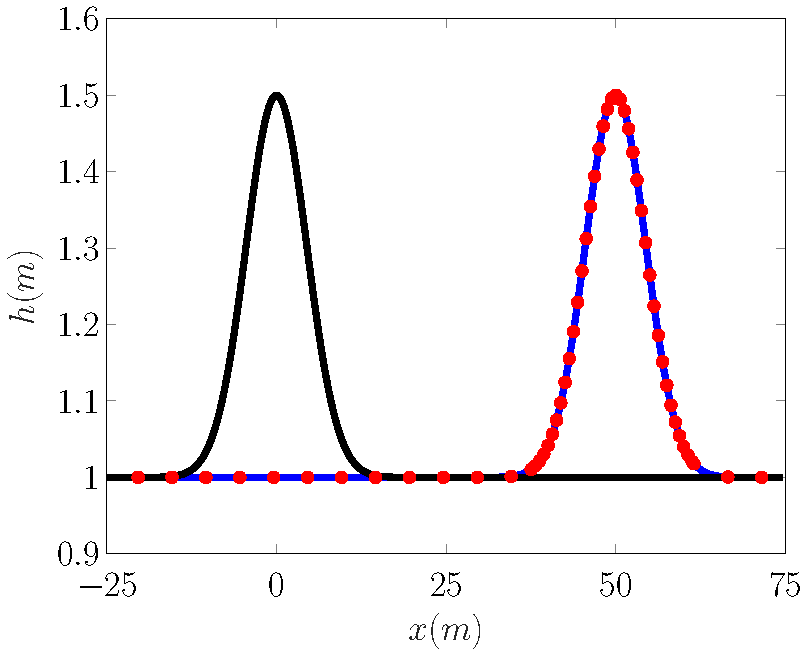
\includegraphics[width=\textwidth]{./Figures/Simulations/Validation/Forced/iSGN/h.pdf}
		\caption{$h$}
	\end{subfigure}
	\begin{subfigure}{0.32\textwidth}
		\centering
		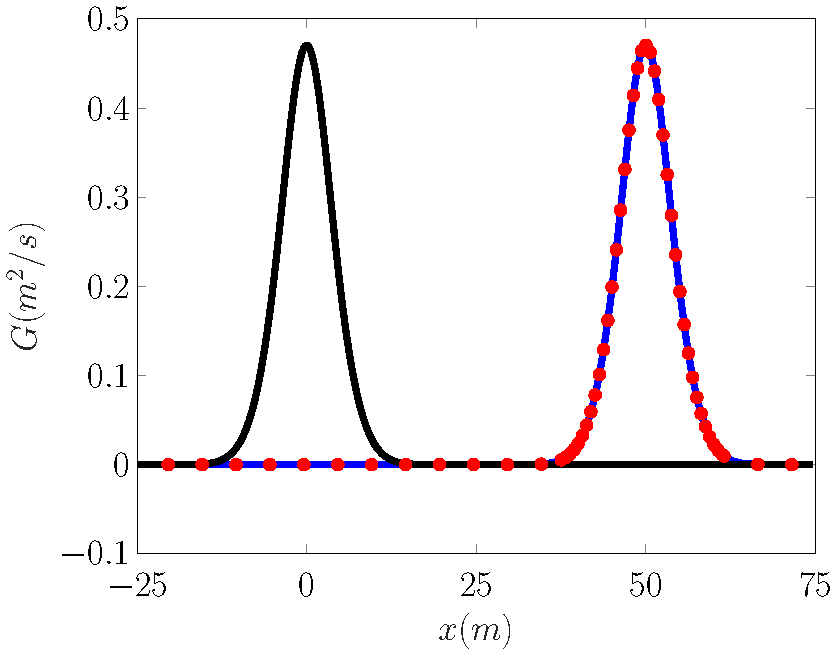
\includegraphics[width=\textwidth]{./Figures/Simulations/Validation/Forced/iSGN//G.pdf}
		\caption{$G$}
	\end{subfigure}
	\begin{subfigure}{0.32\textwidth}
		\centering
		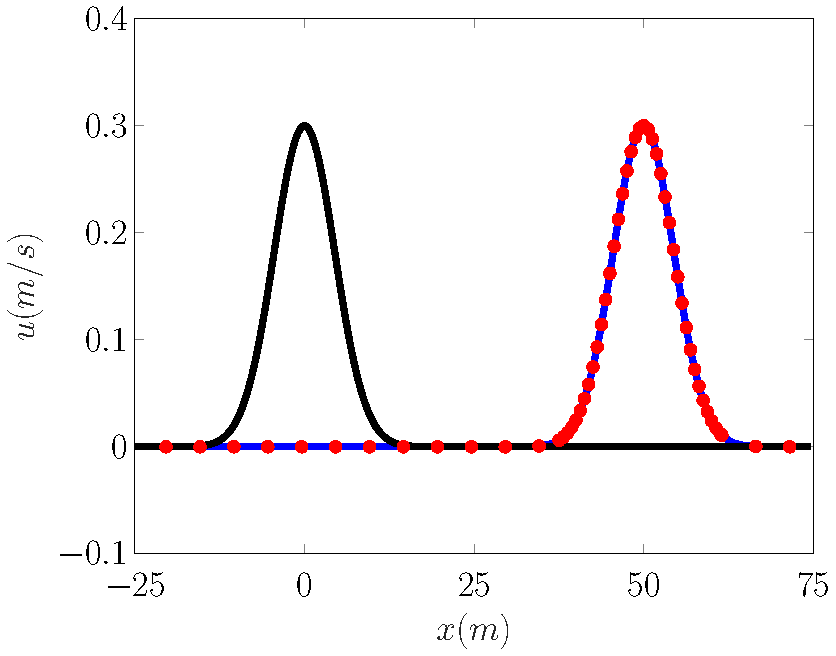
\includegraphics[width=\textwidth]{./Figures/Simulations/Validation/Forced/iSGN/u.pdf}
		\caption{$u$}
	\end{subfigure}
	\caption{Example plots of initial conditions (\solidrule), analytic solution ({\color{blue}\solidrule}), and numerical solution with $\Delta x \approx 0.06m$ (\tikzcircle{red}).}
	\label{Fig:FS_Ex}
\end{figure}

Figure \ref{Fig:FS_Conv} demonstrates the convergence of the numerical scheme as $\Delta x$ decreases. All quantities of interest are converging at the expected second-order. Since the right hand-sides of \eqref{eq:gSGNE_Forced} are evaluated analytically, the observed error is caused by the numerical method alone. Therefore, these results demonstrate that the scheme is second-order for all terms in the gSGNE.
%
\begin{figure}
	\centering
	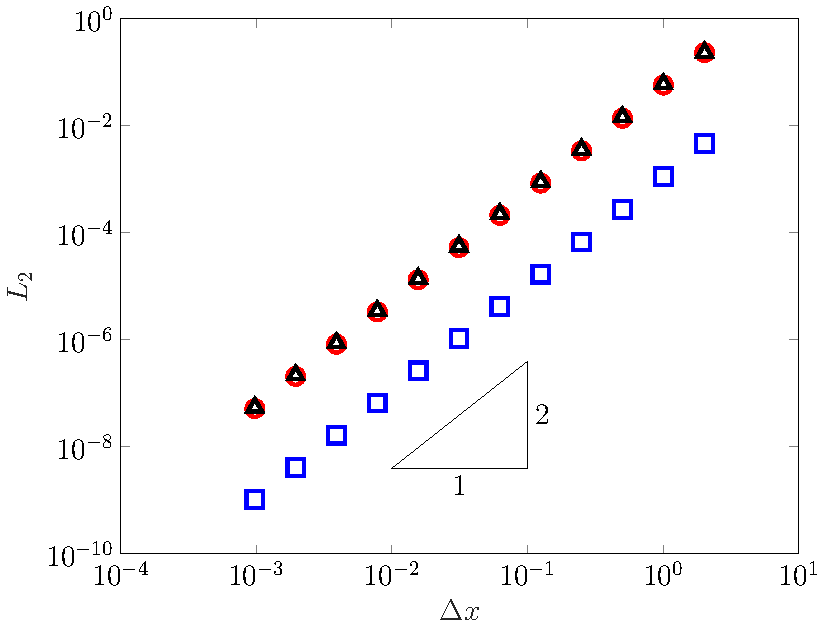
\includegraphics[width=0.49\textwidth]{./Figures/Simulations/Validation/Forced/iSGN/NormResults.pdf}
	\caption{Convergence plot of $h$ (\squaret{blue}) , $G$ (\circlet{red}), $u$ (\trianglet{black}) for the forced solutions for various $\Delta x$ values.}
	\label{Fig:FS_Conv}
\end{figure}


\section{Conclusion}
A modified version of the numerical scheme for the SGNE outlined by \citet{Zoppou-etal-2017} was used to solve the gSGNE \cite{Clamond-Dutykh-2018-237,Clamond-et.al-2017-245}. This numerical scheme for the gSGNE was validated by describing a fully second-order implementation of the numerical method. This numerical method was validated against analytic solutions of the SGNE and SWWE and forced solutions. The analytic solutions demonstrate that the gSGNE solver accurately reproduces important members of the family of equations described by the gSGNE whilst conserving the quantities of interest. The forced solutions demonstrate that the method remains second-order for all values of the free parameters, $\beta_1$ and $\beta_2$. The gSGNE method described above is the first validated numerical method for the gSGNE. Additionally, the described numerical scheme can be straightforwardly extended to higher-order methods as done by \citet{Zoppou-etal-2017} for the SGNE.

\section{References}
\bibliographystyle{unsrtnat}
\bibliography{Bibliography}


\end{document} 